% \appendix\label{appendix:2d_old}
% \appendixpage
% \addappheadtotoc

\begin{appendices}
\chapter*{Appendice}\label{appendix}
\section*{Grafici omessi nel~\Cref{chap:esperimenti}}
Si mostrano in questa appendice i grafici relativi agli esperimenti descritti nel~\Cref{chap:esperimenti} ma precedentemente omessi per ragioni di spazio.
I risultati mostrati nelle seguenti figure sono analoghi a quelli descritti nel~\Cref{chap:esperimenti}, per cui valgono le stesse considerazioni.
La didascalia di ogni figura in questa appendice contiene un riferimento alla figura del~\Cref{chap:esperimenti} che mostra i grafici dello stesso gruppo di esperimenti.

\begin{figure}[b!]
    \centering
    \begin{subfigure}{.8\textwidth}
        \centering
        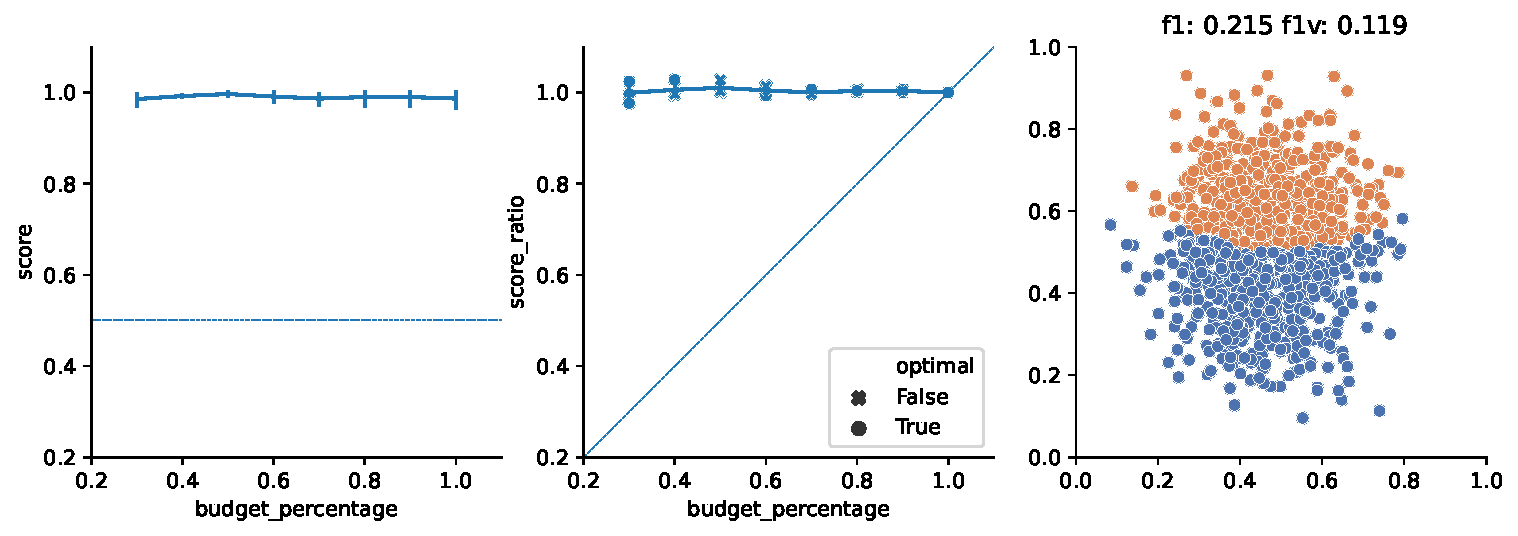
\includegraphics[width=\textwidth]{img/2d/1.pdf}
    \end{subfigure}%
    \hfill
    \begin{subfigure}{.8\textwidth}
        \centering
        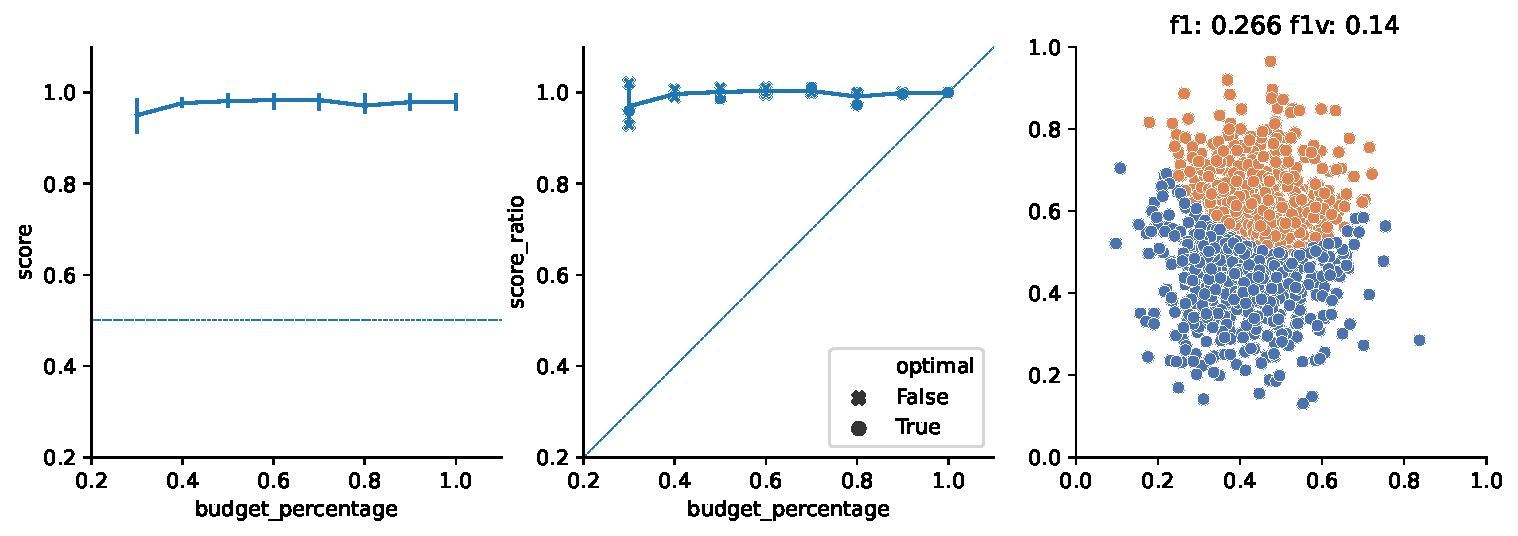
\includegraphics[width=\textwidth]{img/2d/2.pdf}
    \end{subfigure}%
    \hfill
    \begin{subfigure}{.8\textwidth}
        \centering
        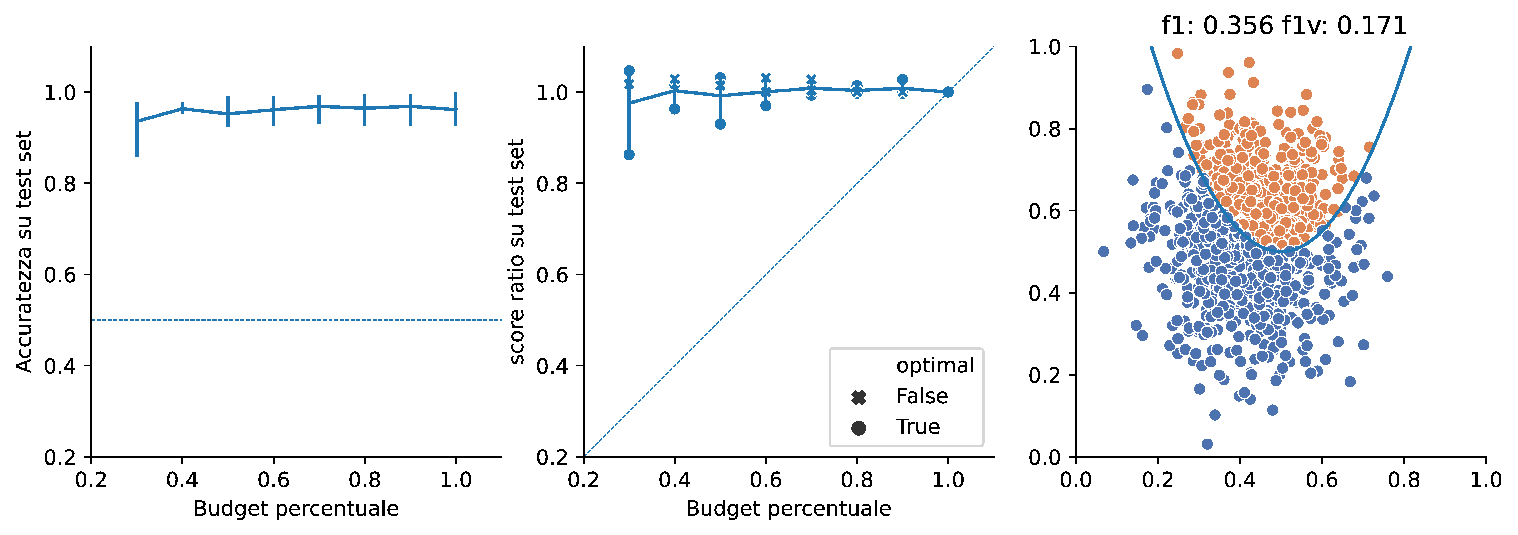
\includegraphics[width=\textwidth]{img/2d/3.pdf}
    \end{subfigure}%
    \caption[Risultati su \emph{dataset} sintetici utilizzando la strategia 1.]{Questi grafici completano la~\Cref{fig:risultati_2d}. Risultati ottenuti su \emph{dataset} sintetici bidimensionali utilizzando la strategia 1. Ognuno dei grafici a sinistra indica l'andamento dell'accuratezza sui dati di \emph{test} al variare del \emph{budget}; ognuno dei grafici al centro indica lo \emph{score ratio} al variare del \emph{budget} (un simbolo ``x'' indica che il risolutore ha prodotto una soluzione non ottima); ognuno dei grafici a destra rappresenta uno dei tre \emph{dataset} utilizzati con le rispettive metriche di difficoltà.}
\end{figure}
\begin{figure}[ht]\ContinuedFloat
    \centering
    \begin{subfigure}{.8\textwidth}
        \centering
        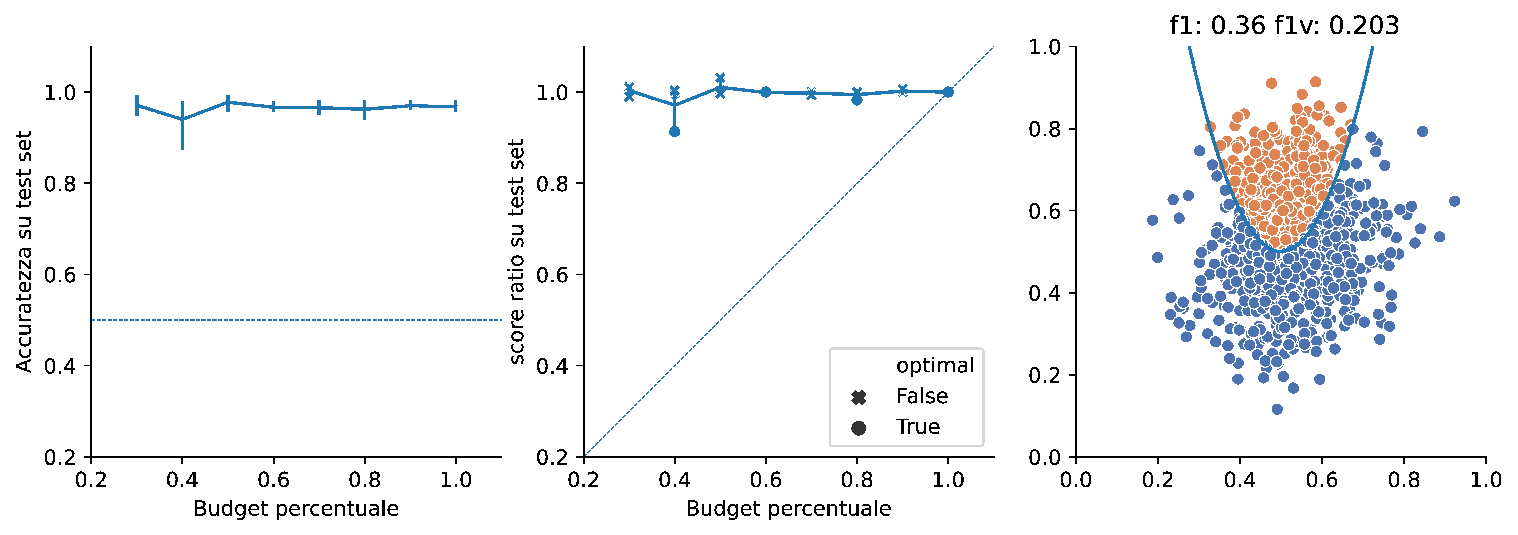
\includegraphics[width=\textwidth]{img/2d/5.pdf}
    \end{subfigure}%
    \hfill
    \begin{subfigure}{.8\textwidth}
        \centering
        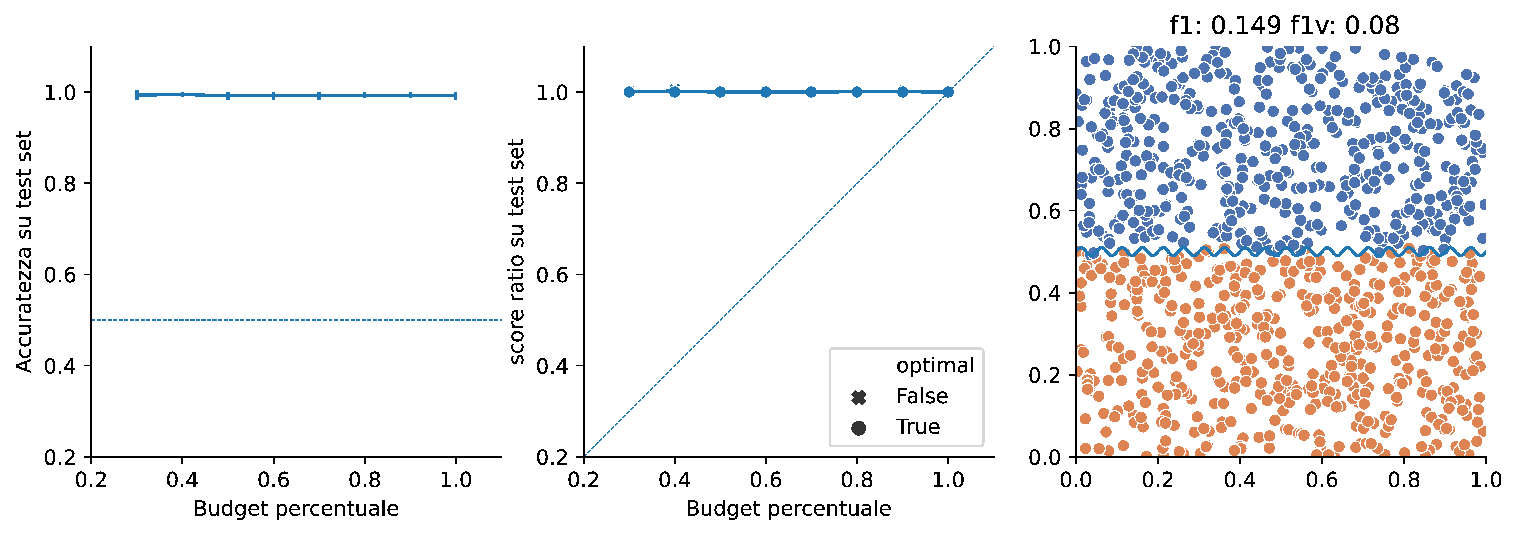
\includegraphics[width=\textwidth]{img/2d/6.pdf}
    \end{subfigure}%
    \hfill
    \begin{subfigure}{.8\textwidth}
        \centering
        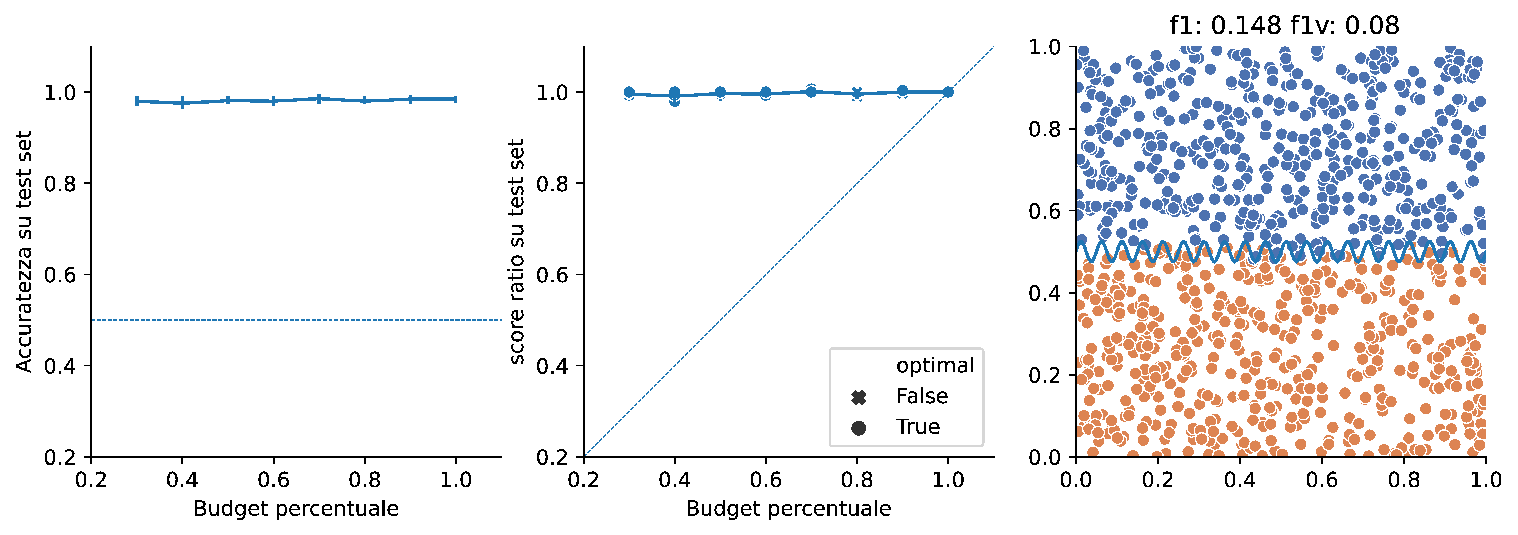
\includegraphics[width=\textwidth]{img/2d/7.pdf}
    \end{subfigure}%
    \hfill
    \begin{subfigure}{.8\textwidth}
        \centering
        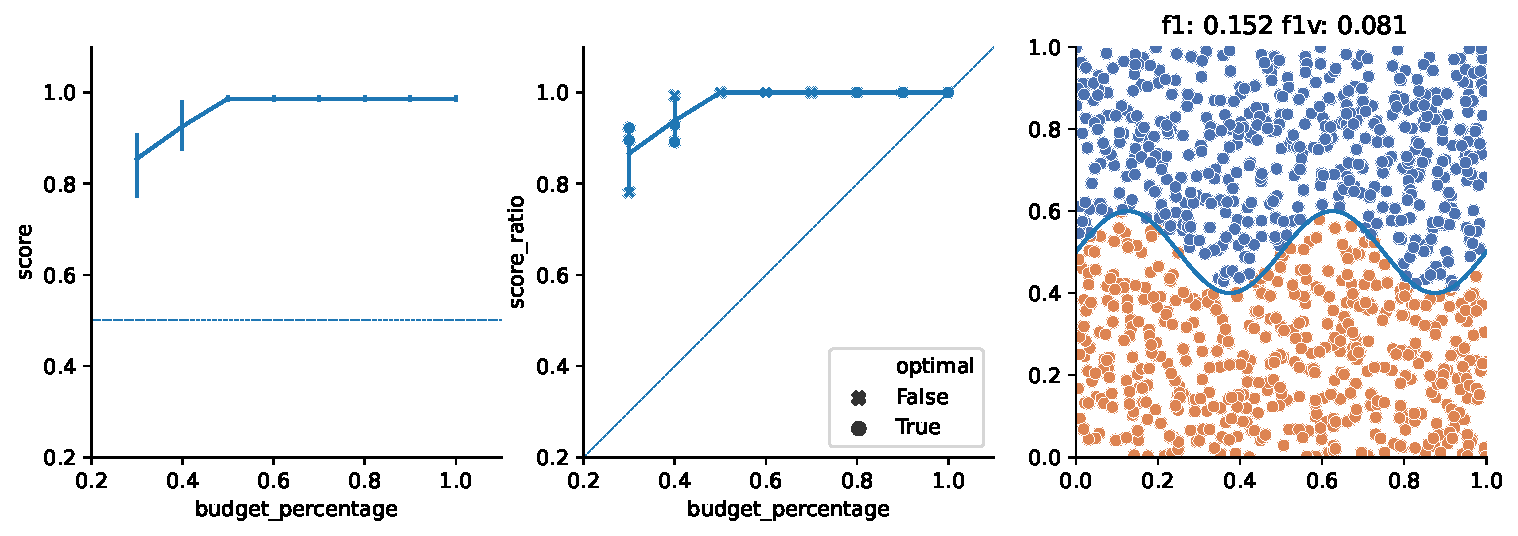
\includegraphics[width=\textwidth]{img/2d/11.pdf}
    \end{subfigure}%
    \caption[Risultati su \emph{dataset} sintetici utilizzando la strategia 1.]{Questi grafici completano la~\Cref{fig:risultati_2d}. Risultati ottenuti su \emph{dataset} sintetici bidimensionali utilizzando la strategia 1. Ognuno dei grafici a sinistra indica l'andamento dell'accuratezza sui dati di \emph{test} al variare del \emph{budget}; ognuno dei grafici al centro indica lo \emph{score ratio} al variare del \emph{budget} (un simbolo ``x'' indica che il risolutore ha prodotto una soluzione non ottima); ognuno dei grafici a destra rappresenta uno dei tre \emph{dataset} utilizzati con le rispettive metriche di difficoltà.}
\end{figure}

\begin{figure}[b!]
    \centering
    \begin{subfigure}{.8\textwidth}
        \centering
        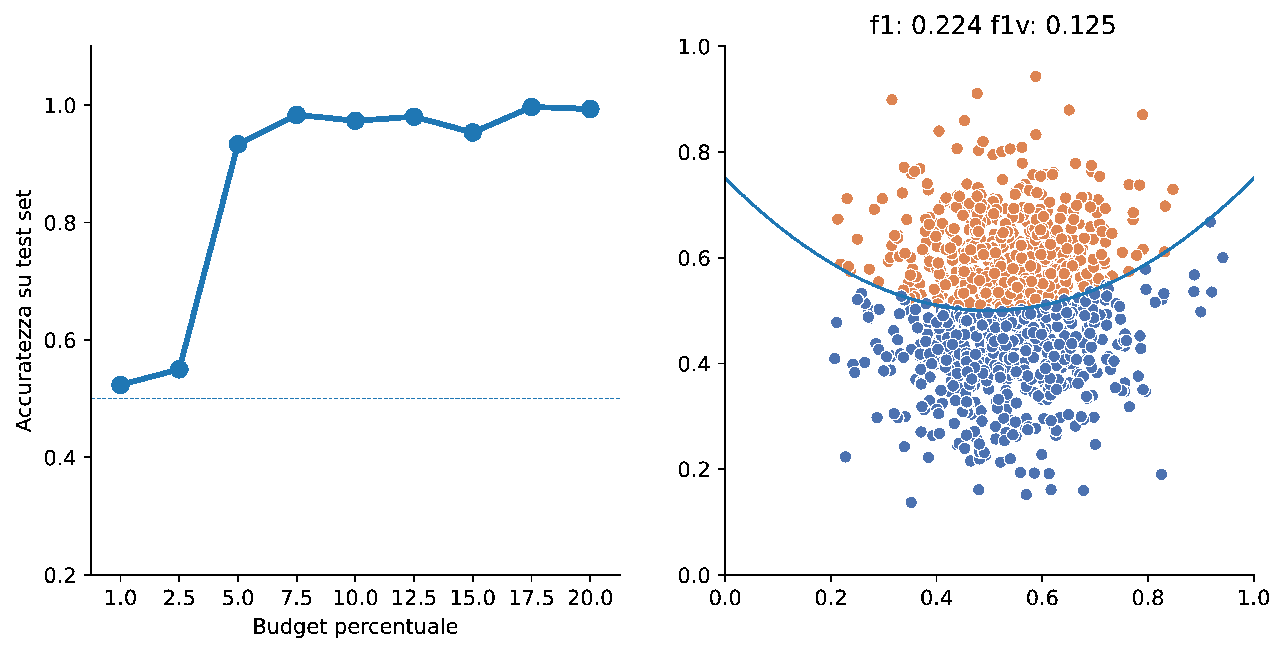
\includegraphics[width=\textwidth]{img/2d_v2/1.pdf}
    \end{subfigure}%
    \hfill
    \begin{subfigure}{.8\textwidth}
        \centering
        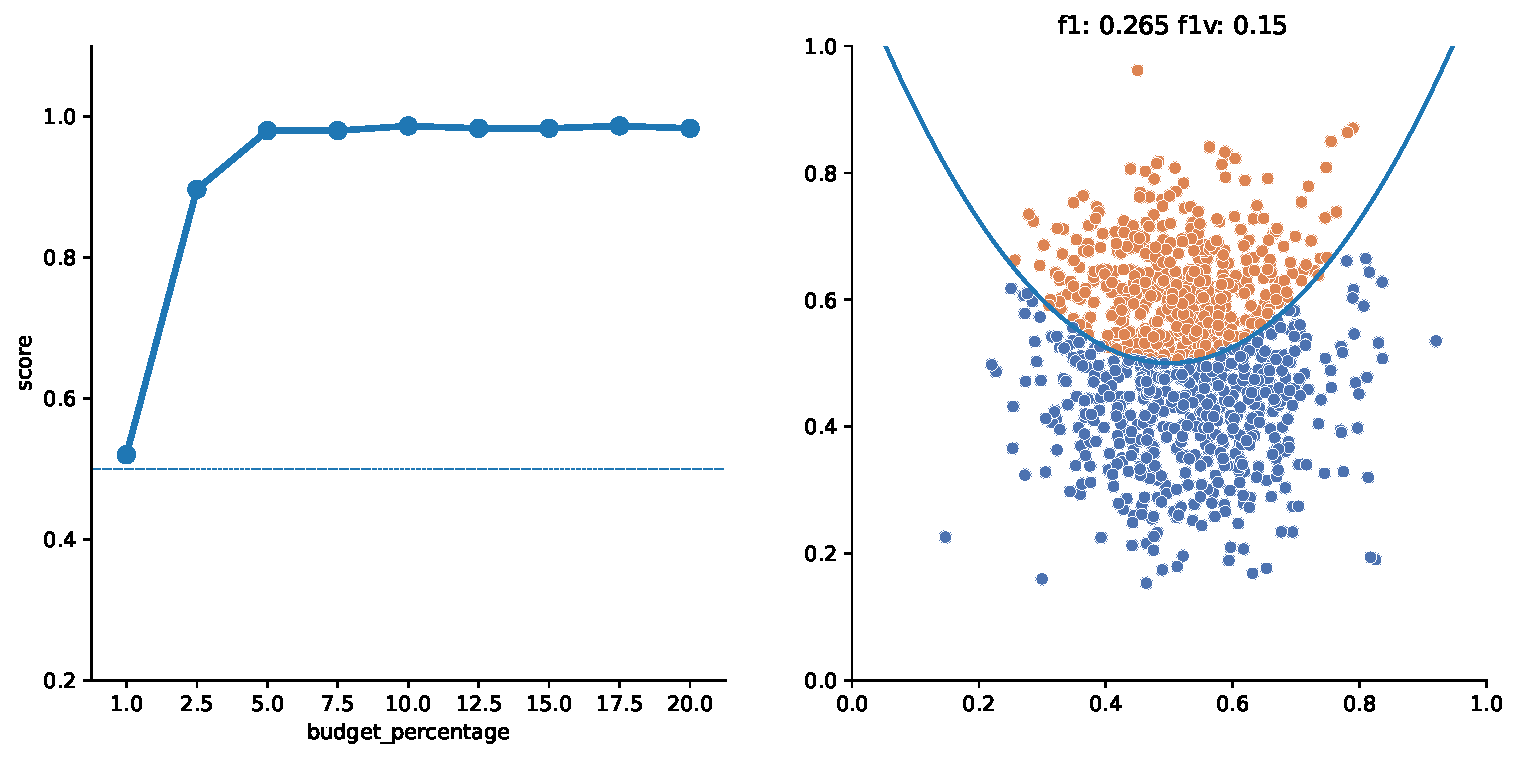
\includegraphics[width=\textwidth]{img/2d_v2/2.pdf}
    \end{subfigure}
    \hfill
    \begin{subfigure}{.8\textwidth}
        \centering
        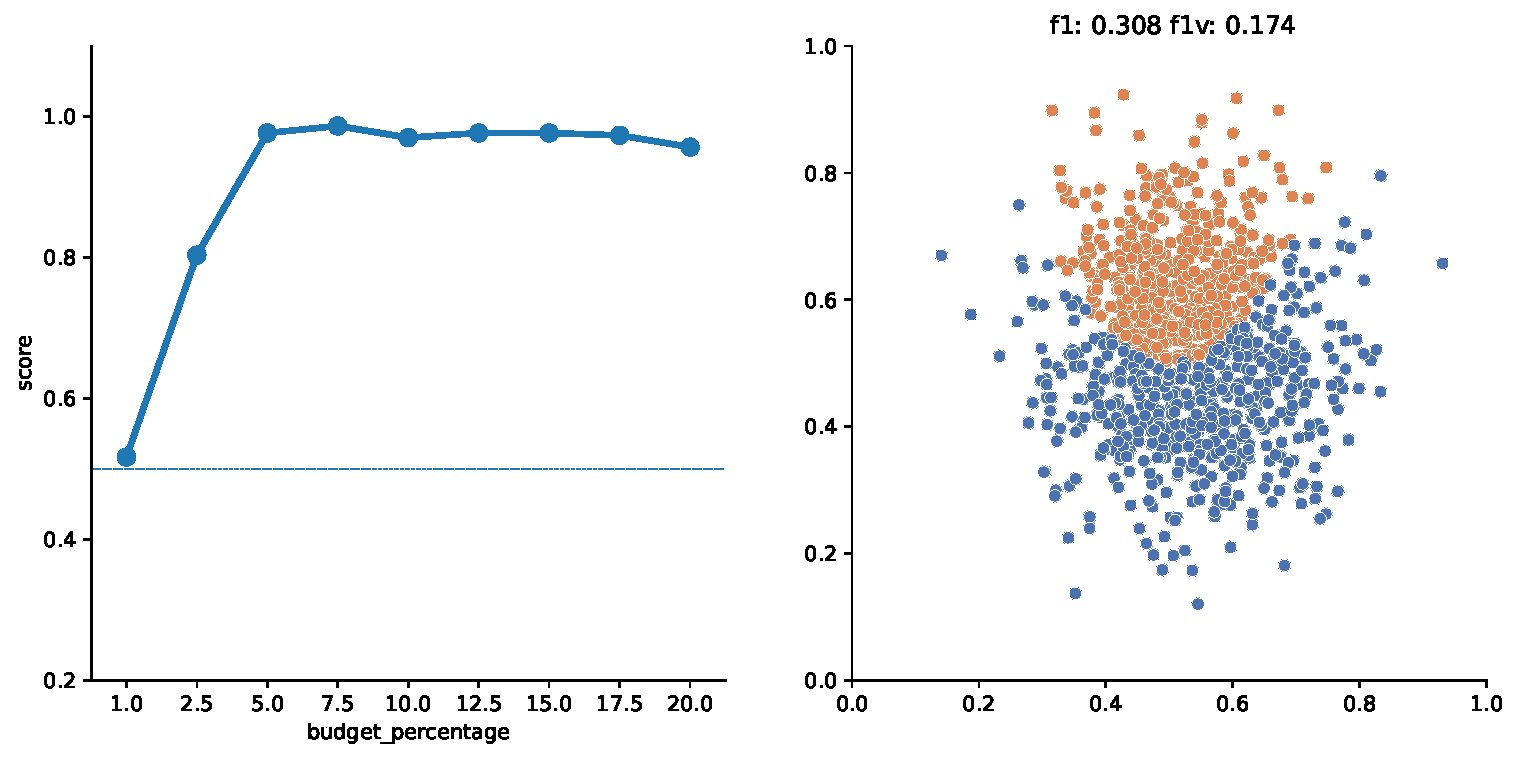
\includegraphics[width=\textwidth]{img/2d_v2/3.pdf}
    \end{subfigure}
    \caption[Risultati su \emph{dataset} sintetici utilizzando la strategia 2.]{Questi grafici completano la~\Cref{fig:2d_v2}. Risultati ottenuti su \emph{dataset} sintetici bidimensionali utilizzando la strategia 2. Ognuno dei grafici a sinistra indica l'andamento dell'accuratezza sui dati di \emph{test} al variare del \emph{budget}; ognuno dei grafici a destra rappresenta il \emph{dataset} utilizzato con le rispettive metriche di difficoltà.}
\end{figure}
\begin{figure}[ht]\ContinuedFloat
    \centering
    \begin{subfigure}{.8\textwidth}
        \centering
        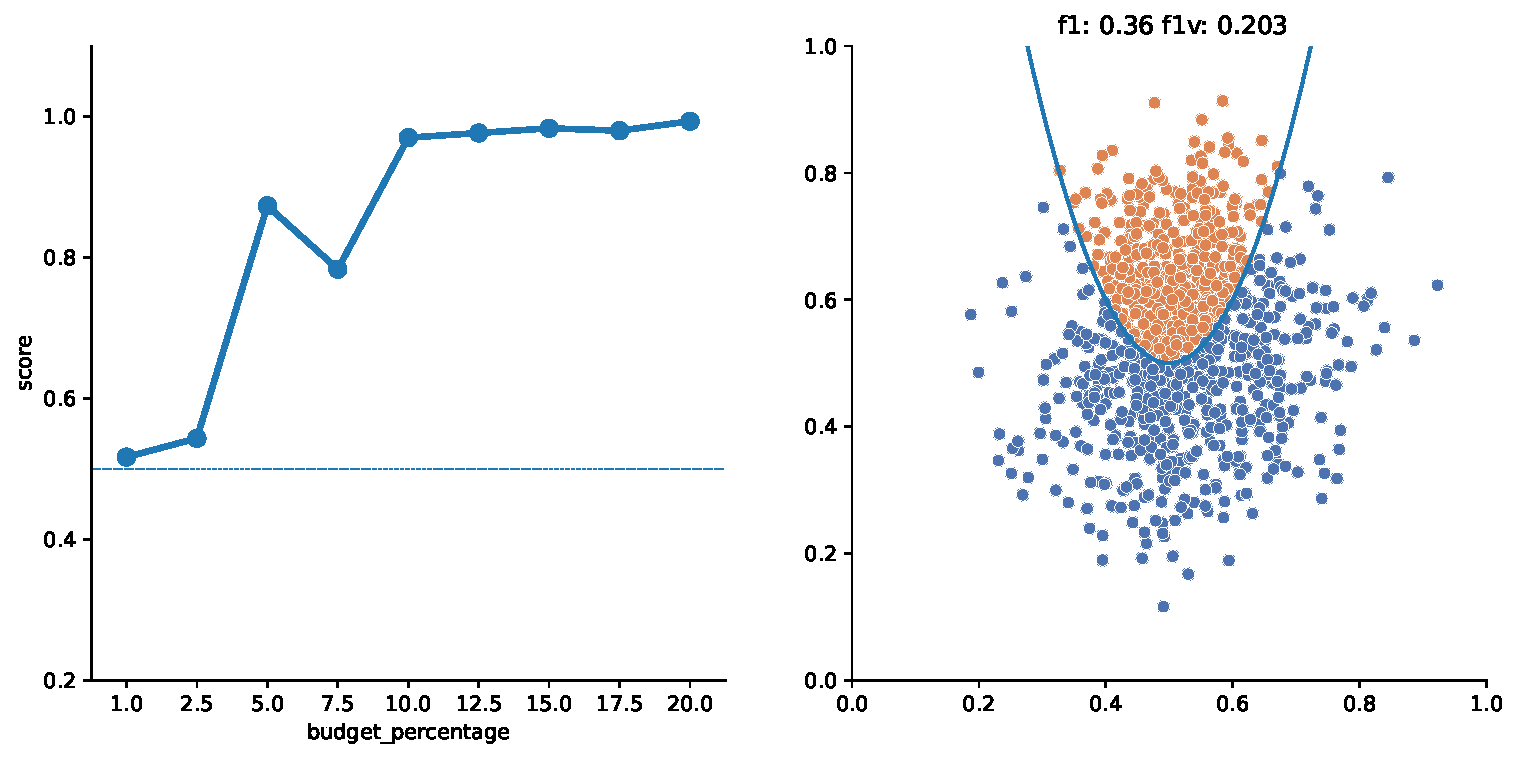
\includegraphics[width=\textwidth]{img/2d_v2/5.pdf}
    \end{subfigure}%
    \hfill
    \begin{subfigure}{.8\textwidth}
        \centering
        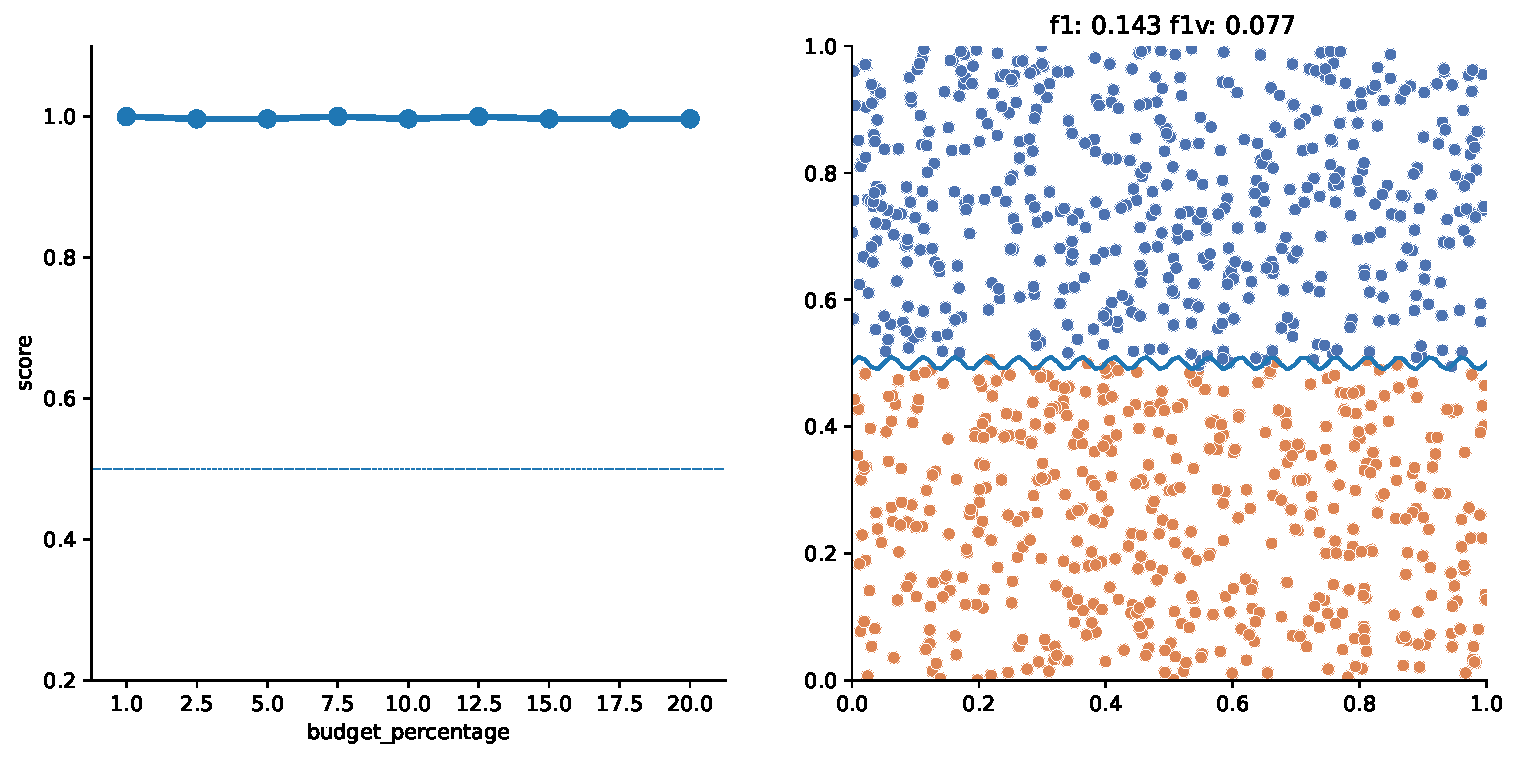
\includegraphics[width=\textwidth]{img/2d_v2/6.pdf}
    \end{subfigure}%
    \hfill
    \begin{subfigure}{.8\textwidth}
        \centering
        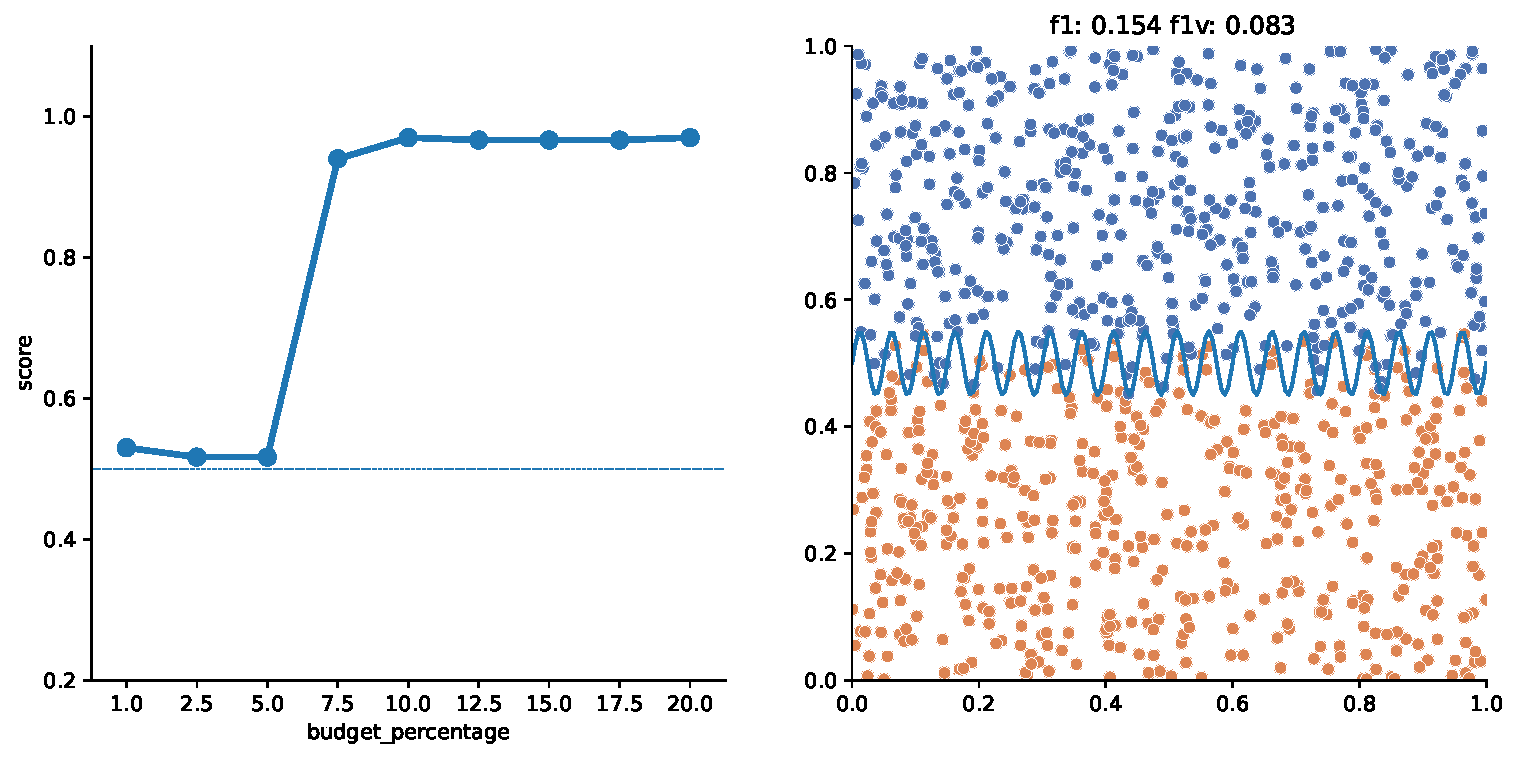
\includegraphics[width=\textwidth]{img/2d_v2/8.pdf}
    \end{subfigure}%
    \caption[Risultati su \emph{dataset} sintetici utilizzando la strategia 2.]{Questi grafici completano la~\Cref{fig:2d_v2}. Risultati ottenuti su \emph{dataset} sintetici bidimensionali utilizzando la strategia 2. Ognuno dei grafici a sinistra indica l'andamento dell'accuratezza sui dati di \emph{test} al variare del \emph{budget}; ognuno dei grafici a destra rappresenta il \emph{dataset} utilizzato con le rispettive metriche di difficoltà.}
\end{figure}
\begin{figure}[ht]\ContinuedFloat
    \centering
    \begin{subfigure}{.8\textwidth}
        \centering
        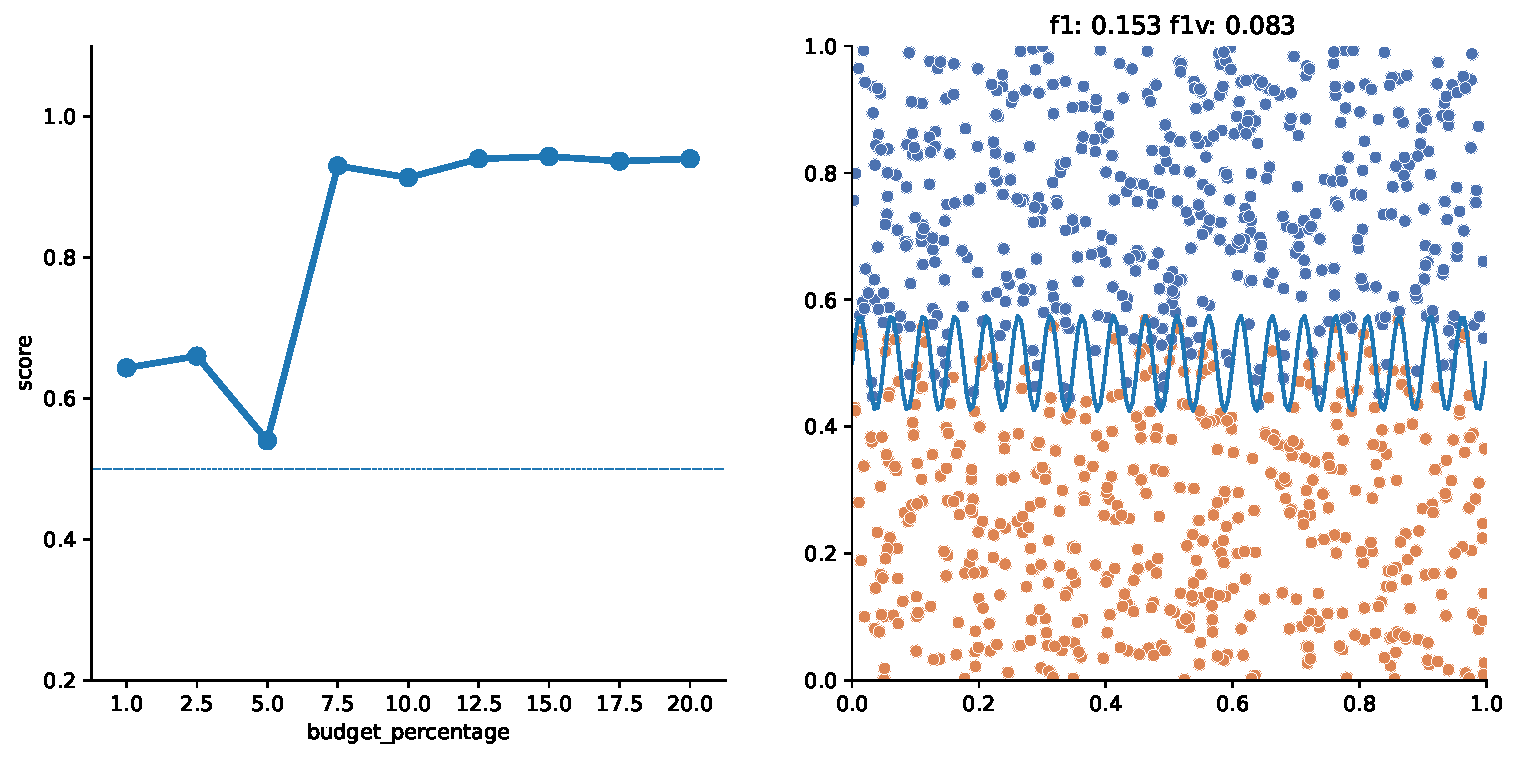
\includegraphics[width=\textwidth]{img/2d_v2/9.pdf}
    \end{subfigure}
    \hfill
    \begin{subfigure}{.8\textwidth}
        \centering
        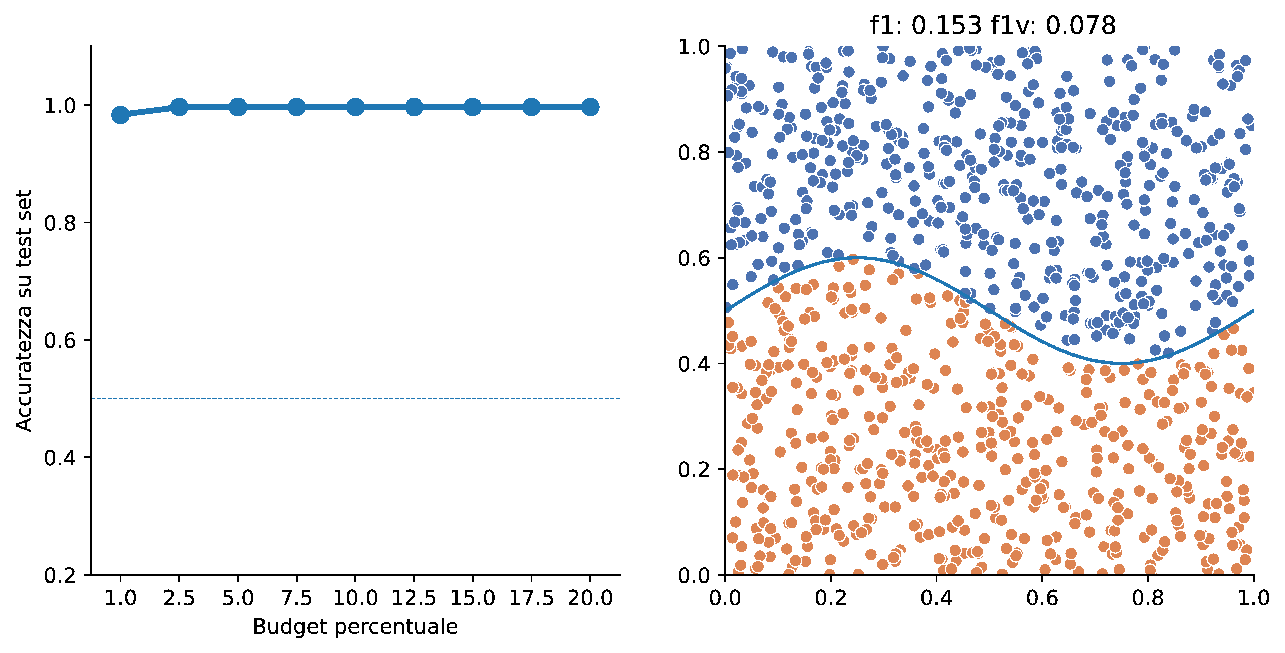
\includegraphics[width=\textwidth]{img/2d_v2/10.pdf}
    \end{subfigure}%
    %
    \hfill
    %Appendice
    \begin{subfigure}{.8\textwidth}
        \centering
        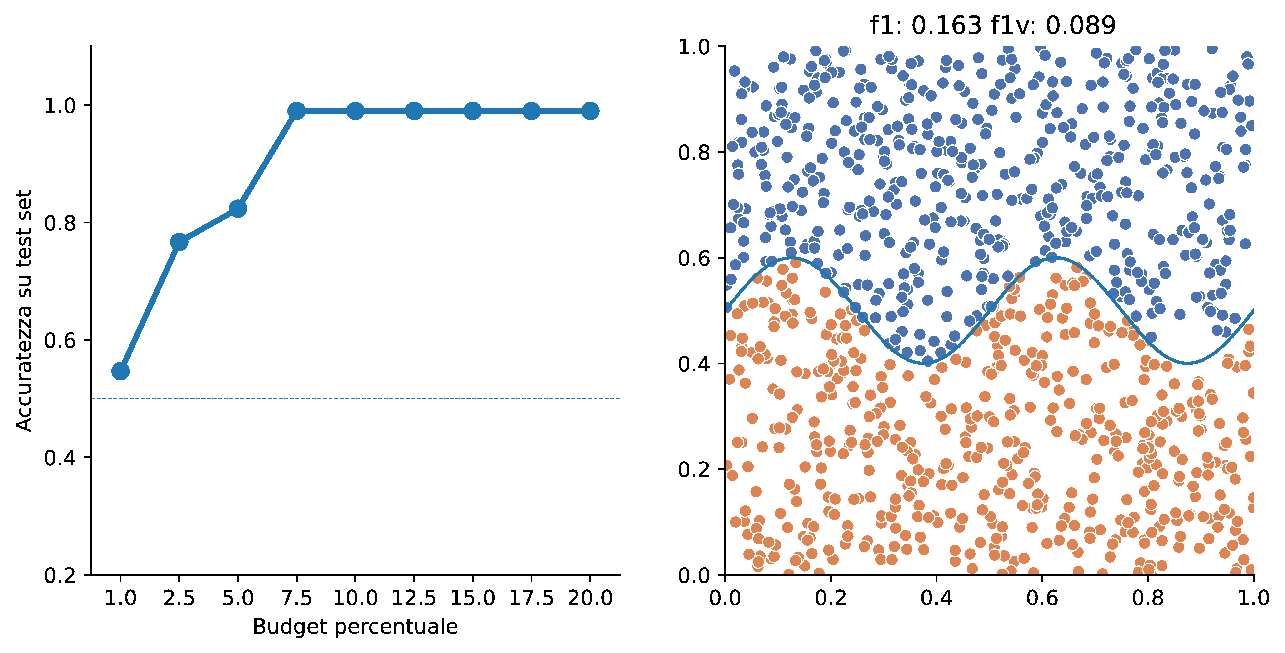
\includegraphics[width=\textwidth]{img/2d_v2/11.pdf}
    \end{subfigure}
    \caption[Risultati su \emph{dataset} sintetici utilizzando la strategia 2.]{Questi grafici completano la~\Cref{fig:2d_v2}. Risultati ottenuti su \emph{dataset} sintetici bidimensionali utilizzando la strategia 2. Ognuno dei grafici a sinistra indica l'andamento dell'accuratezza sui dati di \emph{test} al variare del \emph{budget}; ognuno dei grafici a destra rappresenta il \emph{dataset} utilizzato con le rispettive metriche di difficoltà.}
\end{figure}


\begin{figure}[b!]
\centering
    \begin{subfigure}{.8\textwidth}
        \centering
        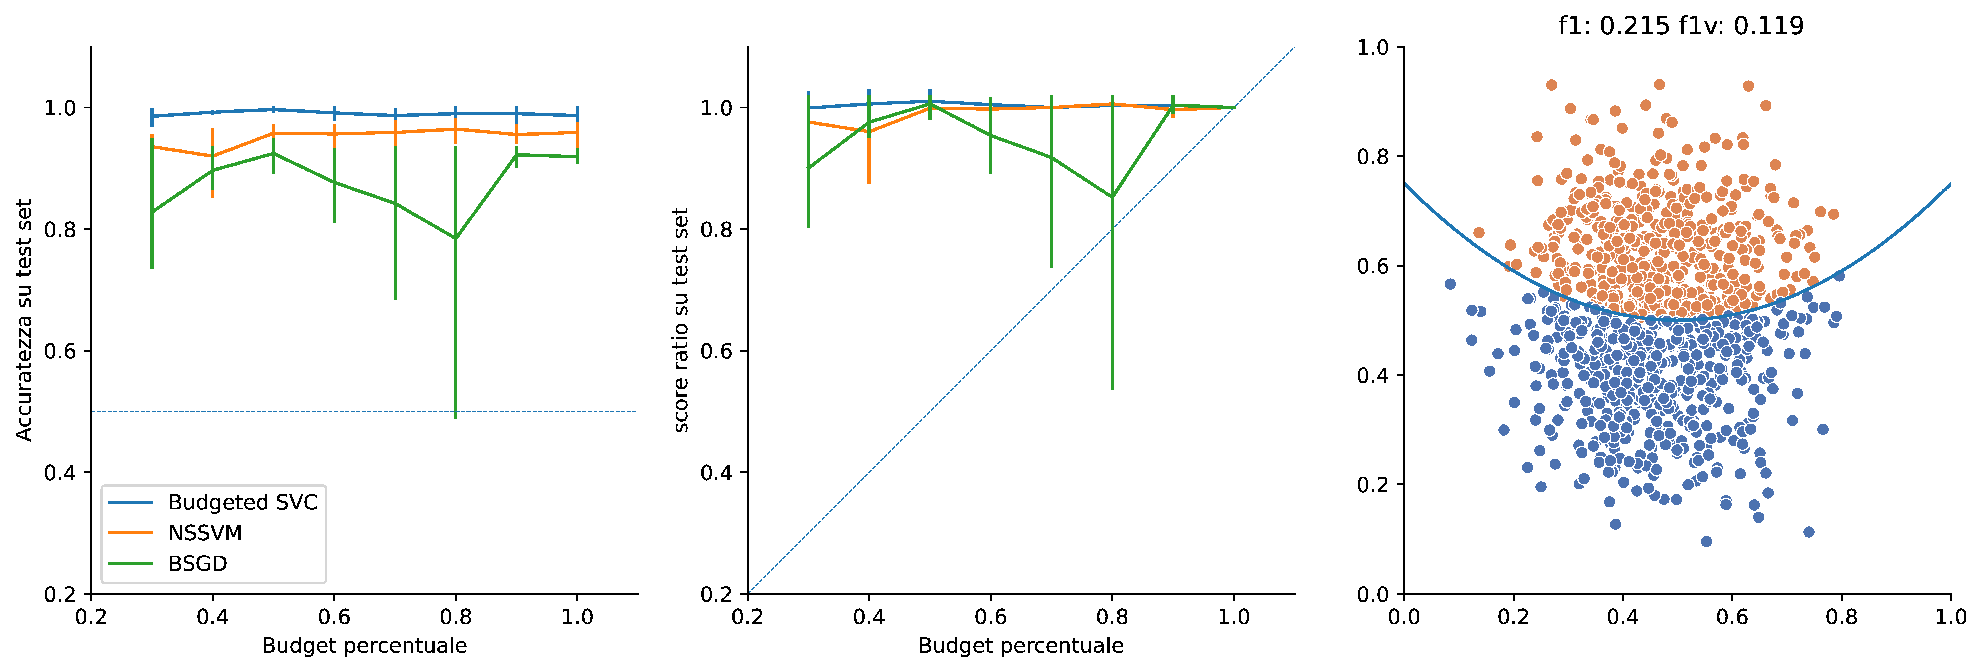
\includegraphics[width=\textwidth]{img/comp_old/1.pdf}
    \end{subfigure}%
    \hfill
    \begin{subfigure}{.8\textwidth}
        \centering
        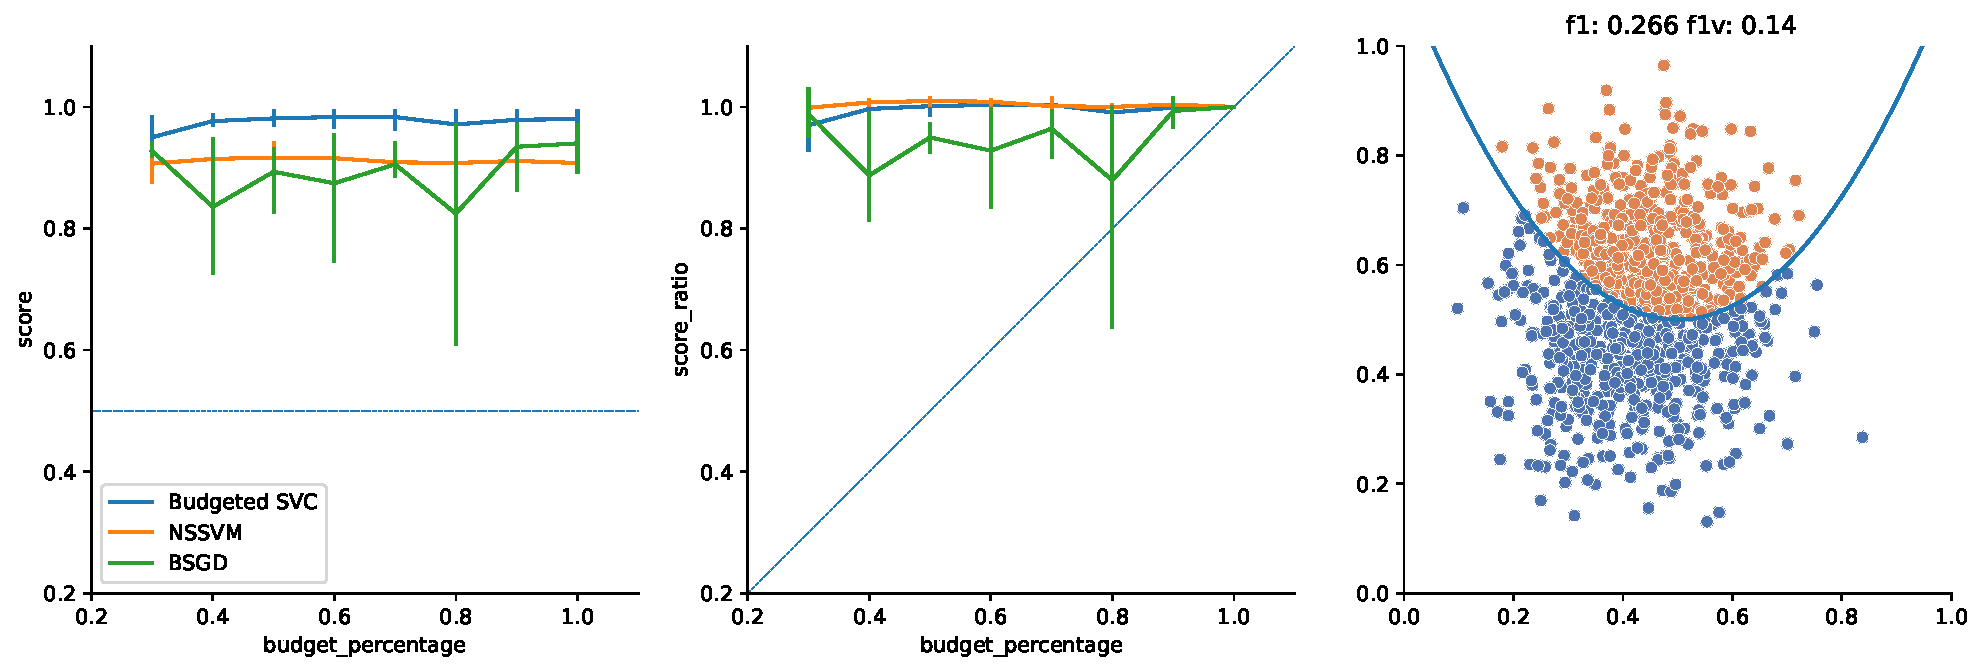
\includegraphics[width=\textwidth]{img/comp_old/2.pdf}
    \end{subfigure}
    \hfill
    \begin{subfigure}{.8\textwidth}
        \centering
        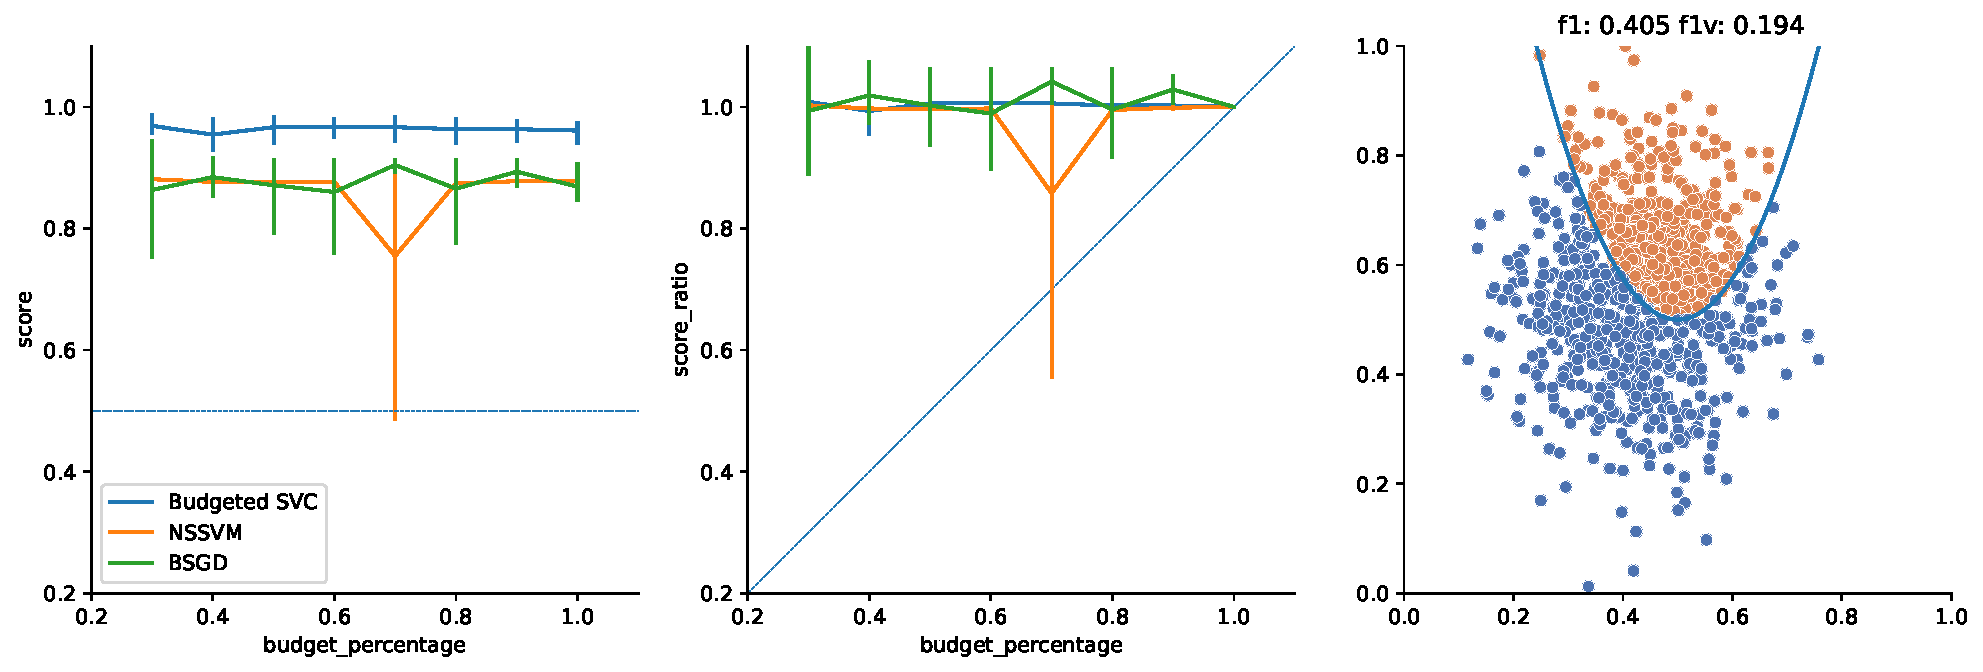
\includegraphics[width=\textwidth]{img/comp_old/4.pdf}
    \end{subfigure}
    \hfill
    \begin{subfigure}{.8\textwidth}
        \centering
        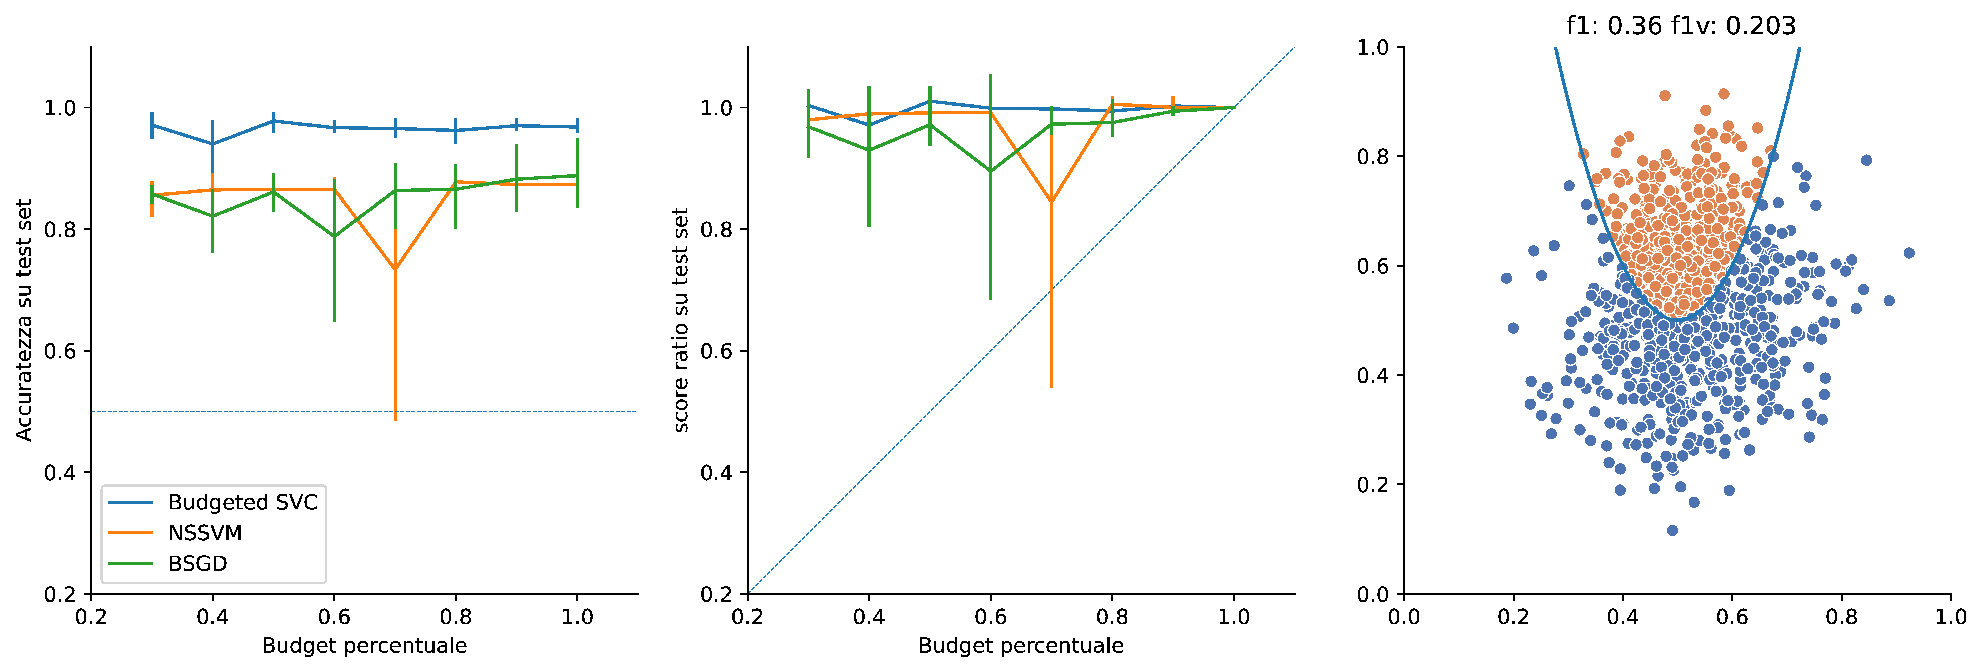
\includegraphics[width=\textwidth]{img/comp_old/5.pdf}
    \end{subfigure}
    \caption[Risultati su \emph{dataset} sintetici utilizzando strategia 1 in confronto ad altri metodi.]{Questi grafici completano la~\Cref{fig:comp_old}. Risultati ottenuti su \emph{dataset} sintetici bidimensionali utilizzando la strategia 1, analogo ai risultati in~\Cref{fig:risultati_2d} ma con una curva per ogni metodo utilizzato: la proposta \emph{Budgeted SVC}, i metodi \emph{NSSVM} e \emph{BSGD}.}
\end{figure}
\begin{figure}[ht]\ContinuedFloat
    \centering
    \begin{subfigure}{.8\textwidth}
        \centering
        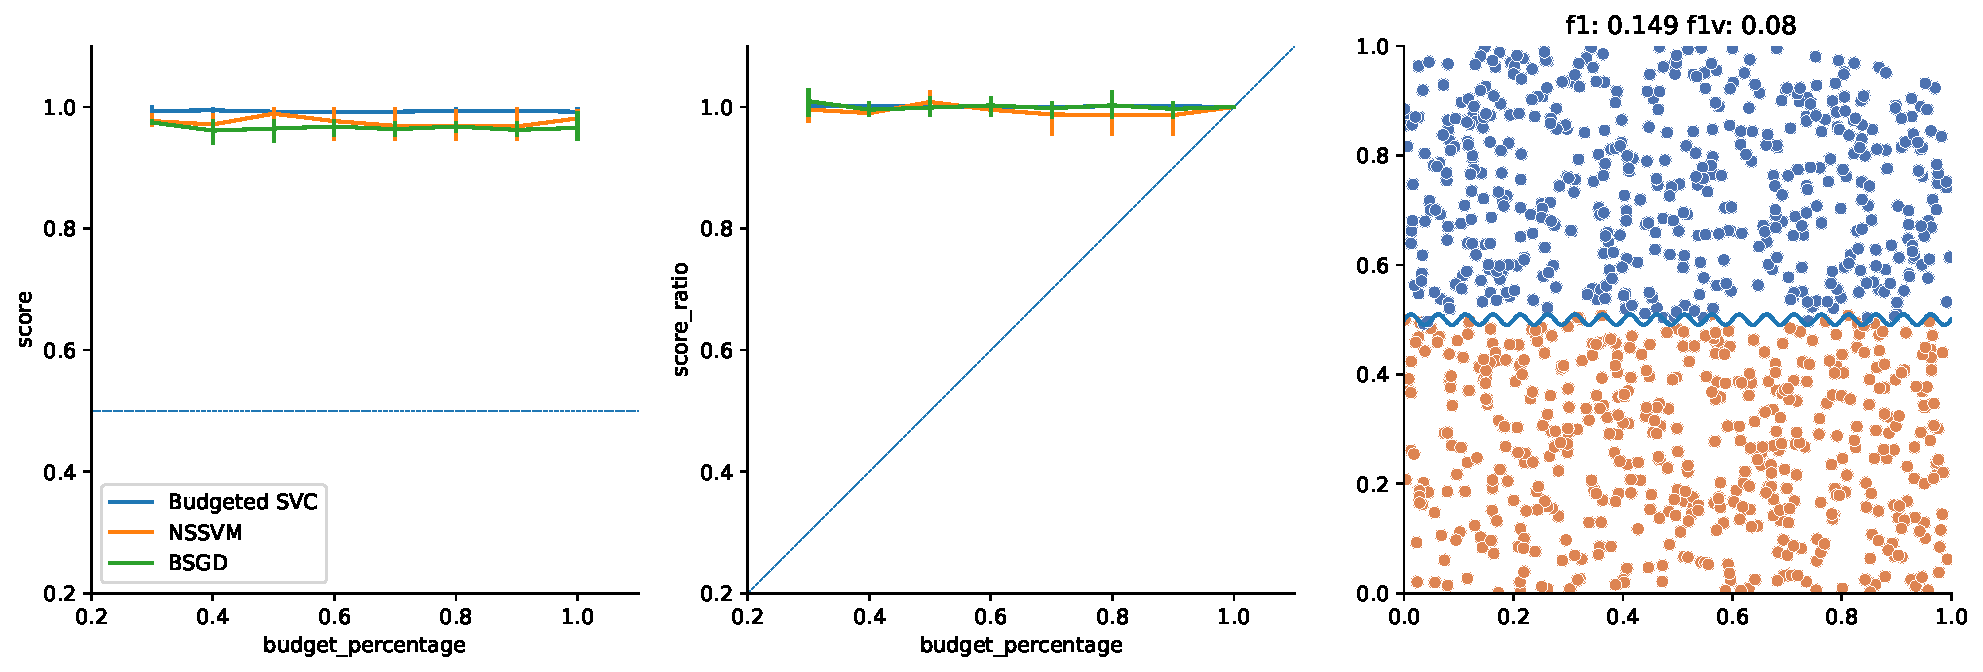
\includegraphics[width=\textwidth]{img/comp_old/6.pdf}
    \end{subfigure}%
    \hfill
    \begin{subfigure}{.8\textwidth}
        \centering
        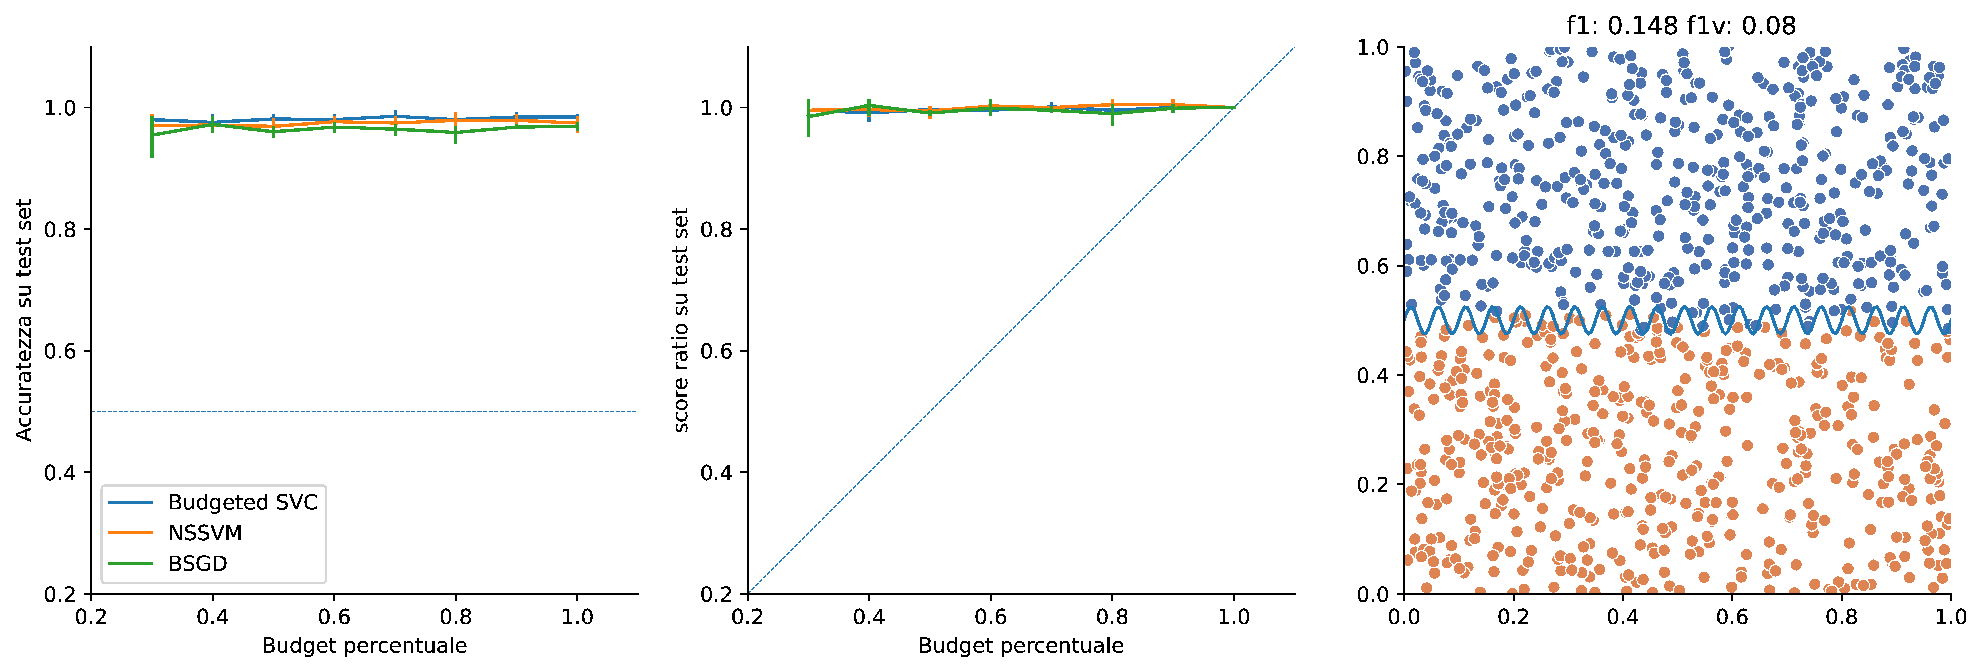
\includegraphics[width=\textwidth]{img/comp_old/7.pdf}
    \end{subfigure}
    \hfill
    \begin{subfigure}{.8\textwidth}
        \centering
        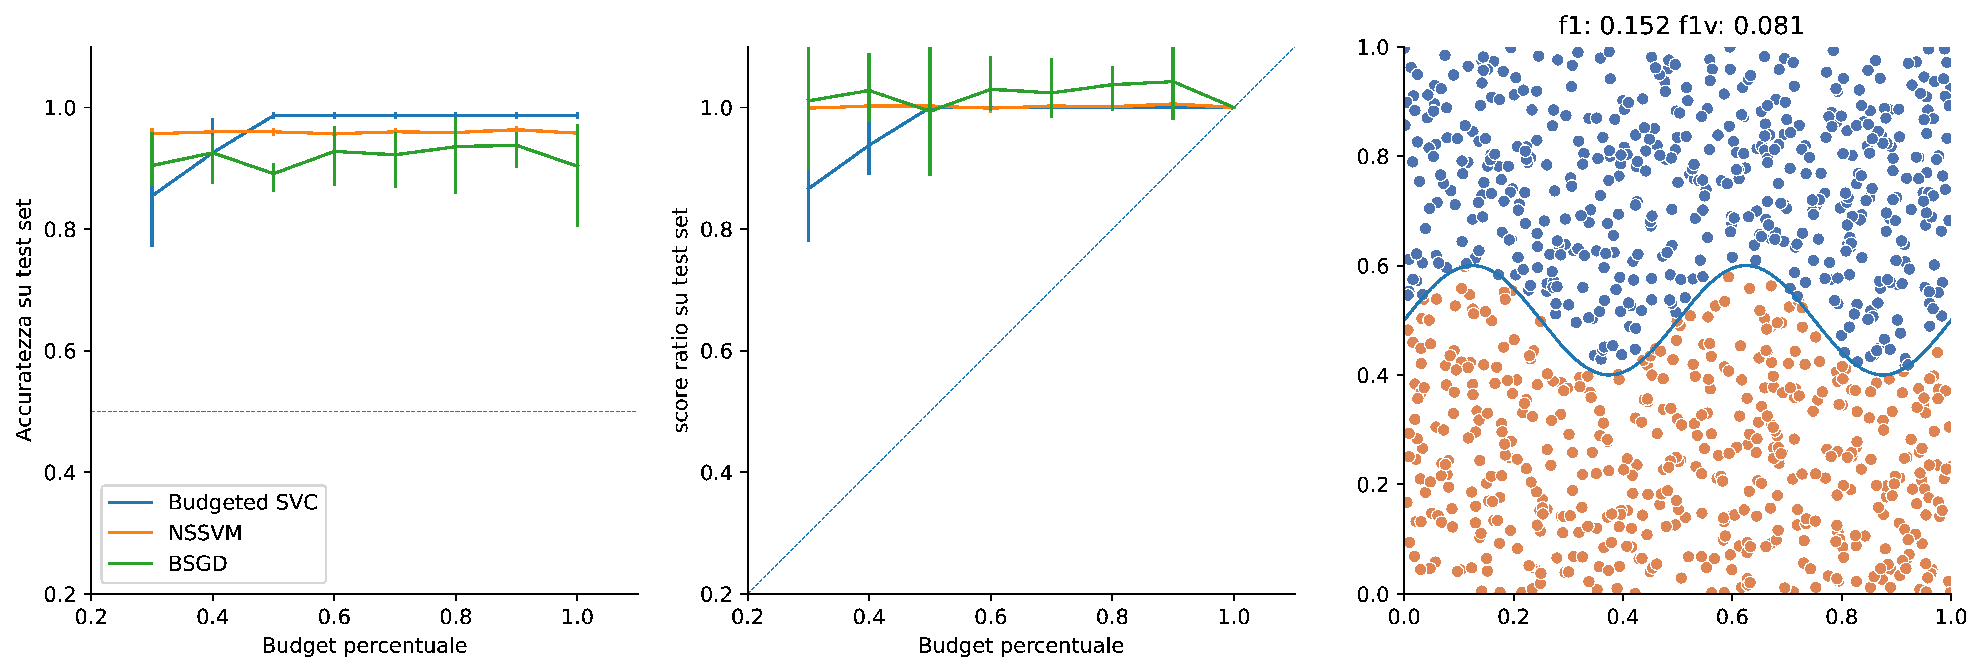
\includegraphics[width=\textwidth]{img/comp_old/11.pdf}
    \end{subfigure}%
    \caption[Risultati su \emph{dataset} sintetici utilizzando strategia 1 in confronto ad altri metodi.]{Questi grafici completano la~\Cref{fig:comp_old}. Risultati ottenuti su \emph{dataset} sintetici bidimensionali utilizzando la strategia 1, analogo ai risultati in~\Cref{fig:risultati_2d} ma con una curva per ogni metodo utilizzato: la proposta \emph{Budgeted SVC}, i metodi \emph{NSSVM} e \emph{BSGD}.}
\end{figure}

\begin{figure}
\centering
    \begin{subfigure}{.8\textwidth}
        \centering
        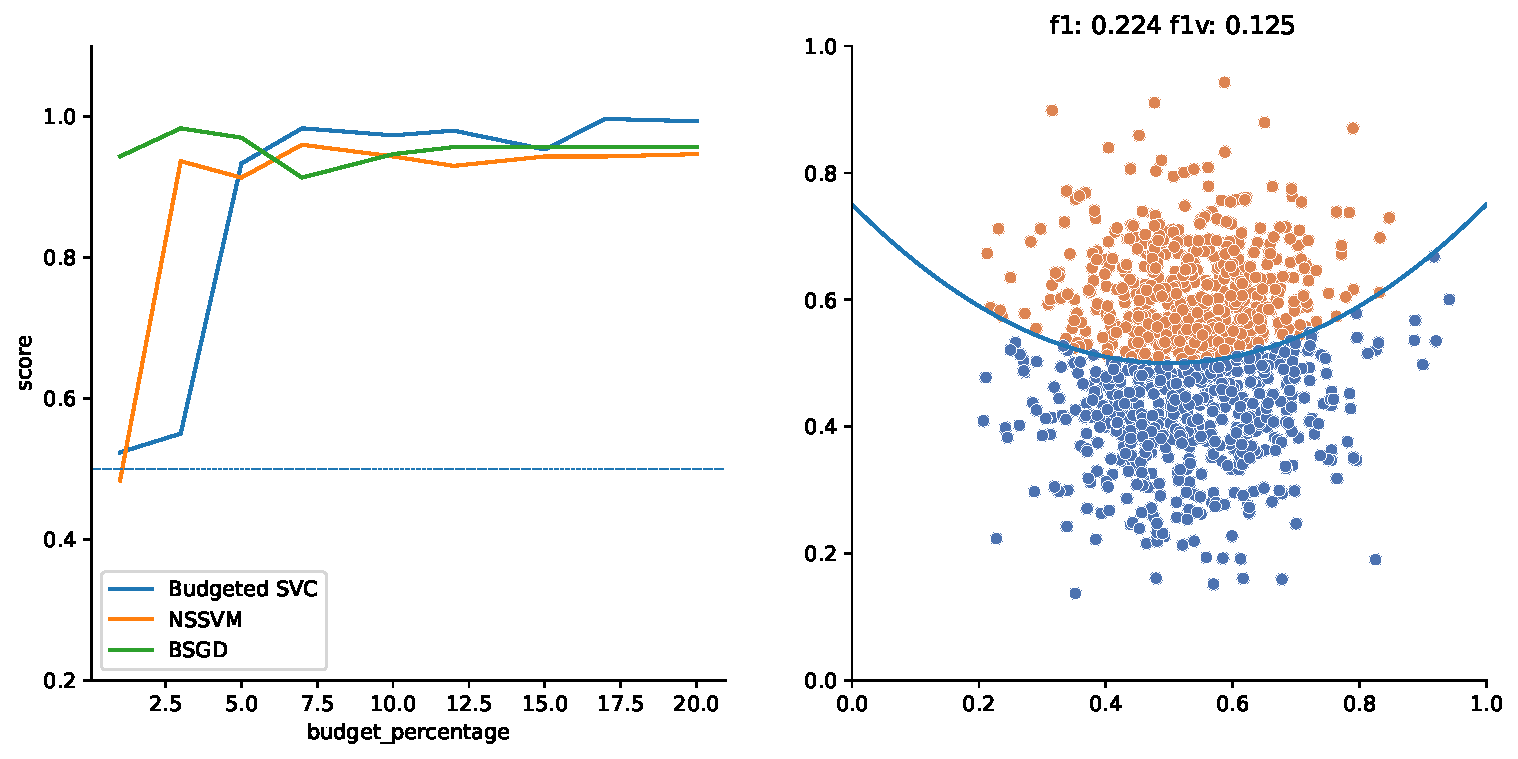
\includegraphics[width=\textwidth]{img/comp_new/1.pdf}
    \end{subfigure}
    \hfill
    \begin{subfigure}{.8\textwidth}
        \centering
        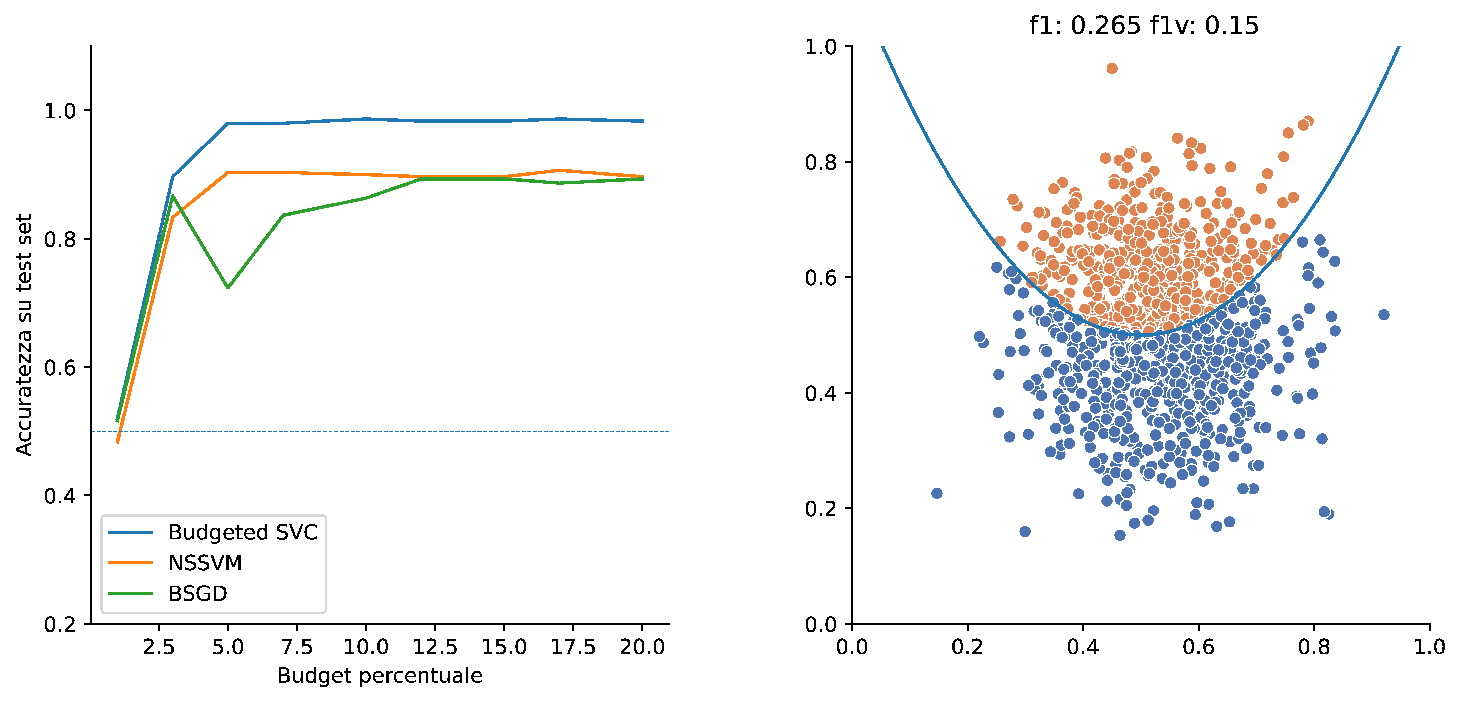
\includegraphics[width=\textwidth]{img/comp_new/2.pdf}
    \end{subfigure}
    \hfill
    \begin{subfigure}{.8\textwidth}
        \centering
        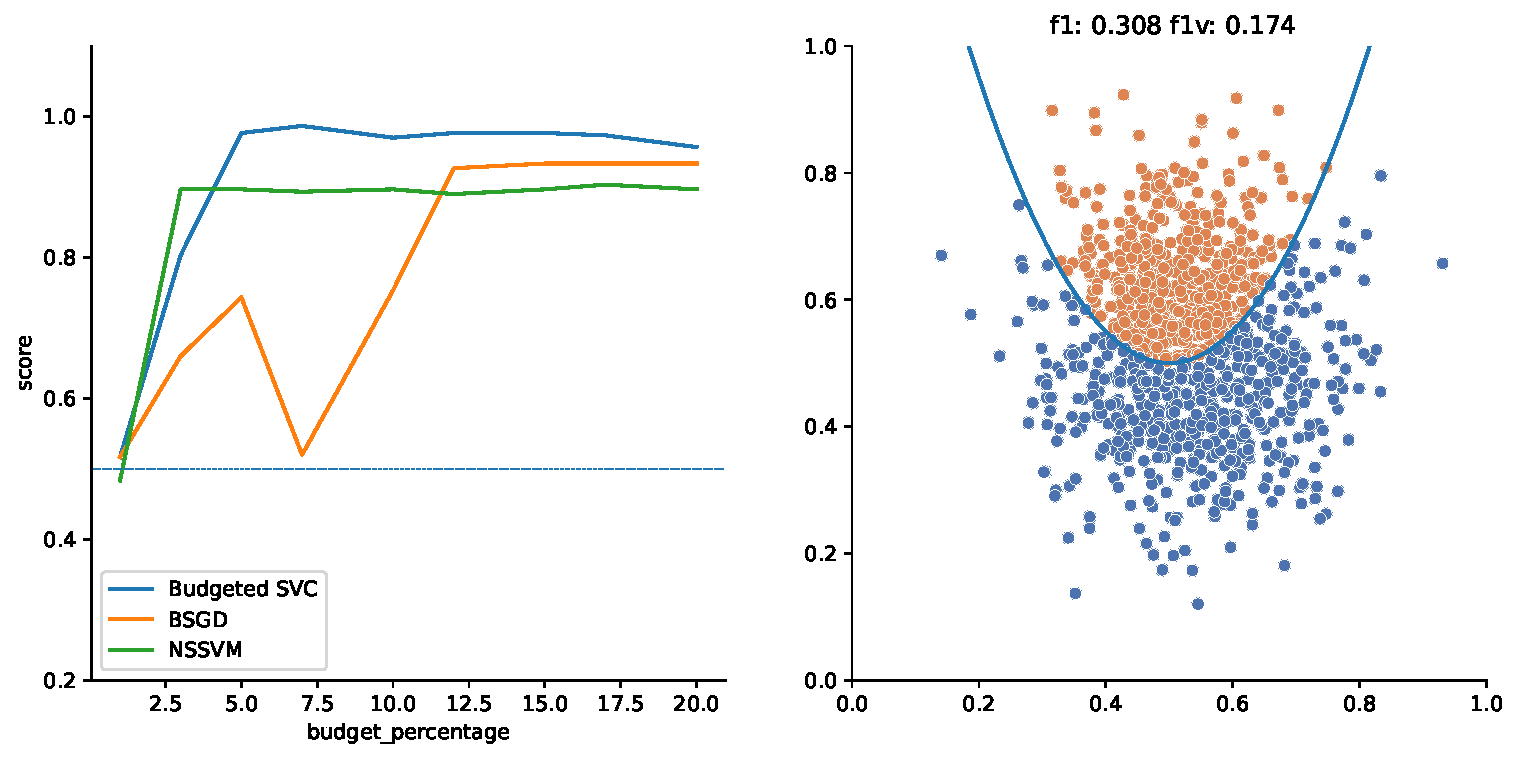
\includegraphics[width=\textwidth]{img/comp_new/3.pdf}
    \end{subfigure}
     \caption[Risultati su \emph{dataset} sintetici utilizzando strategia 2 in confronto ad altri metodi.]{Questi grafici completano la~\Cref{fig:comp_new}. Risultati ottenuti su \emph{dataset} sintetici bidimensionali utilizzando la strategia 2, analogo ai risultati in~\Cref{fig:2d_v2} ma con una curva per ogni metodo utilizzato: la proposta \emph{Budgeted SVC}, i metodi \emph{NSSVM} e \emph{BSGD}.}
\end{figure}
\begin{figure}[ht]\ContinuedFloat
\centering
    \begin{subfigure}{.8\textwidth}
        \centering
        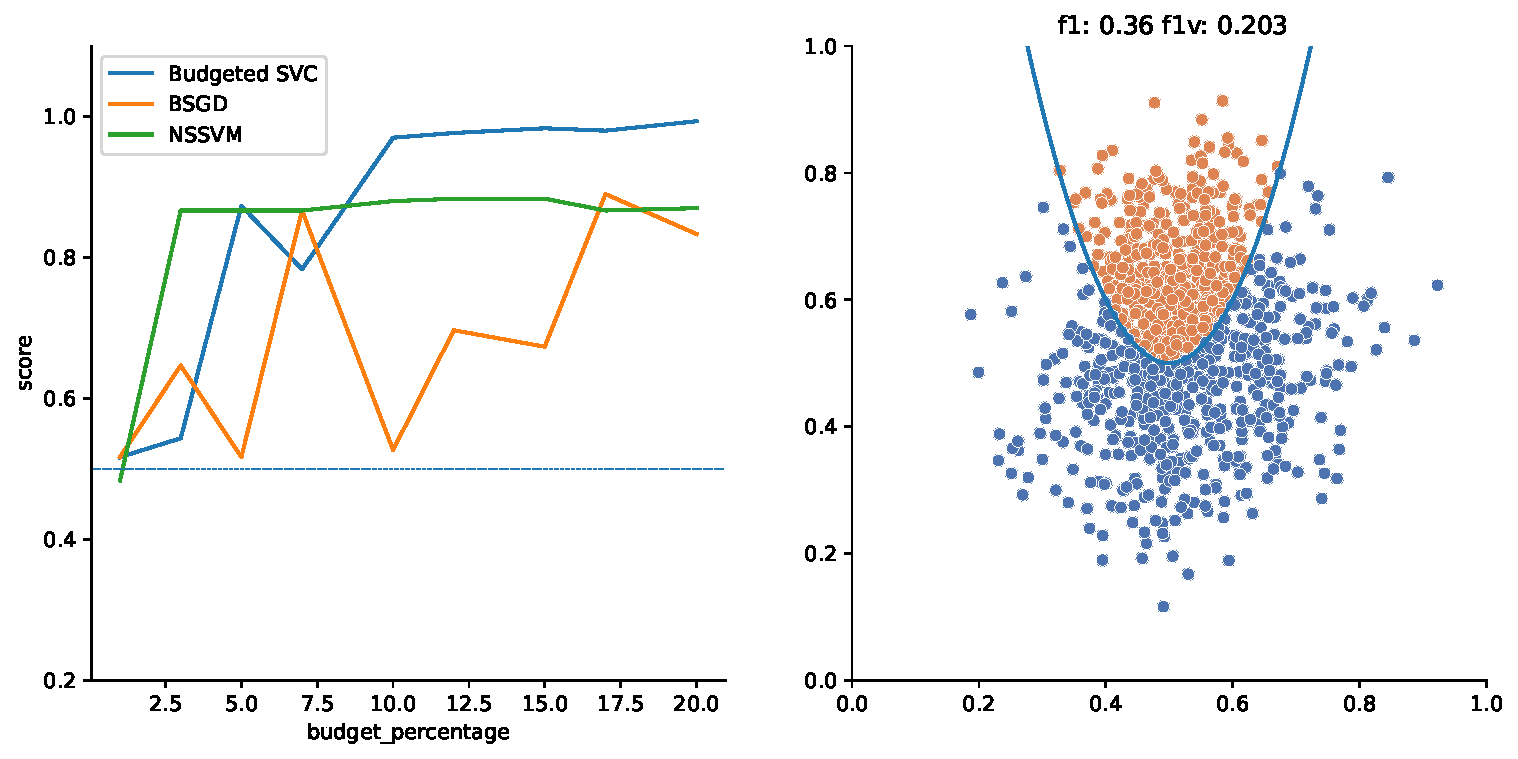
\includegraphics[width=\textwidth]{img/comp_new/5.pdf}
    \end{subfigure}%
    \hfill
    \begin{subfigure}{.8\textwidth}
        \centering
        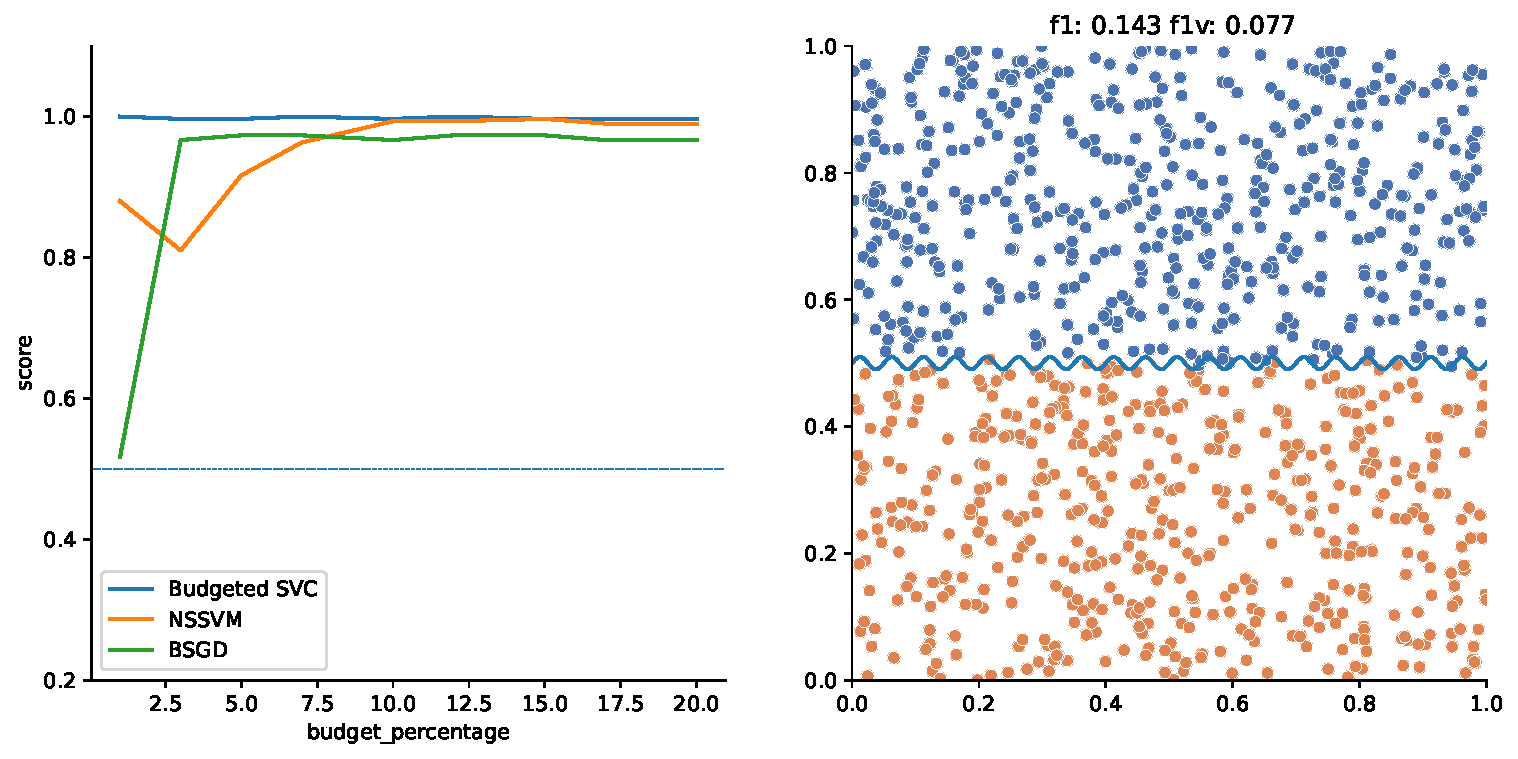
\includegraphics[width=\textwidth]{img/comp_new/6.pdf}
    \end{subfigure}%
    \hfill
    \begin{subfigure}{.8\textwidth}
        \centering
        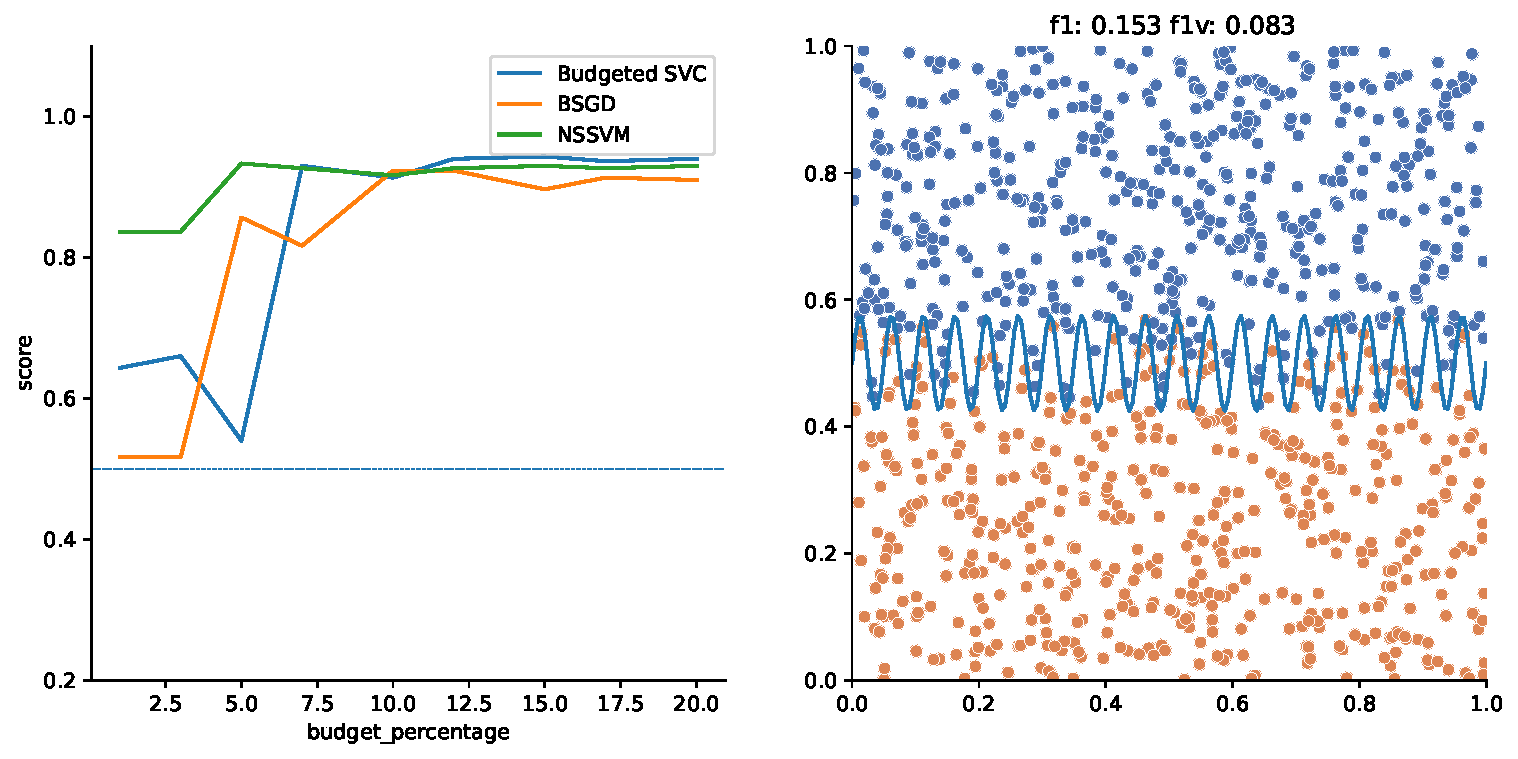
\includegraphics[width=\textwidth]{img/comp_new/9.pdf}
    \end{subfigure}
     \caption[Risultati su \emph{dataset} sintetici utilizzando strategia 2 in confronto ad altri metodi.]{Questi grafici completano la~\Cref{fig:comp_new}. Risultati ottenuti su \emph{dataset} sintetici bidimensionali utilizzando la strategia 2, analogo ai risultati in~\Cref{fig:2d_v2} ma con una curva per ogni metodo utilizzato: la proposta \emph{Budgeted SVC}, i metodi \emph{NSSVM} e \emph{BSGD}.}
\end{figure}
\begin{figure}[ht]\ContinuedFloat
    \centering
    \begin{subfigure}{.8\textwidth}
        \centering
        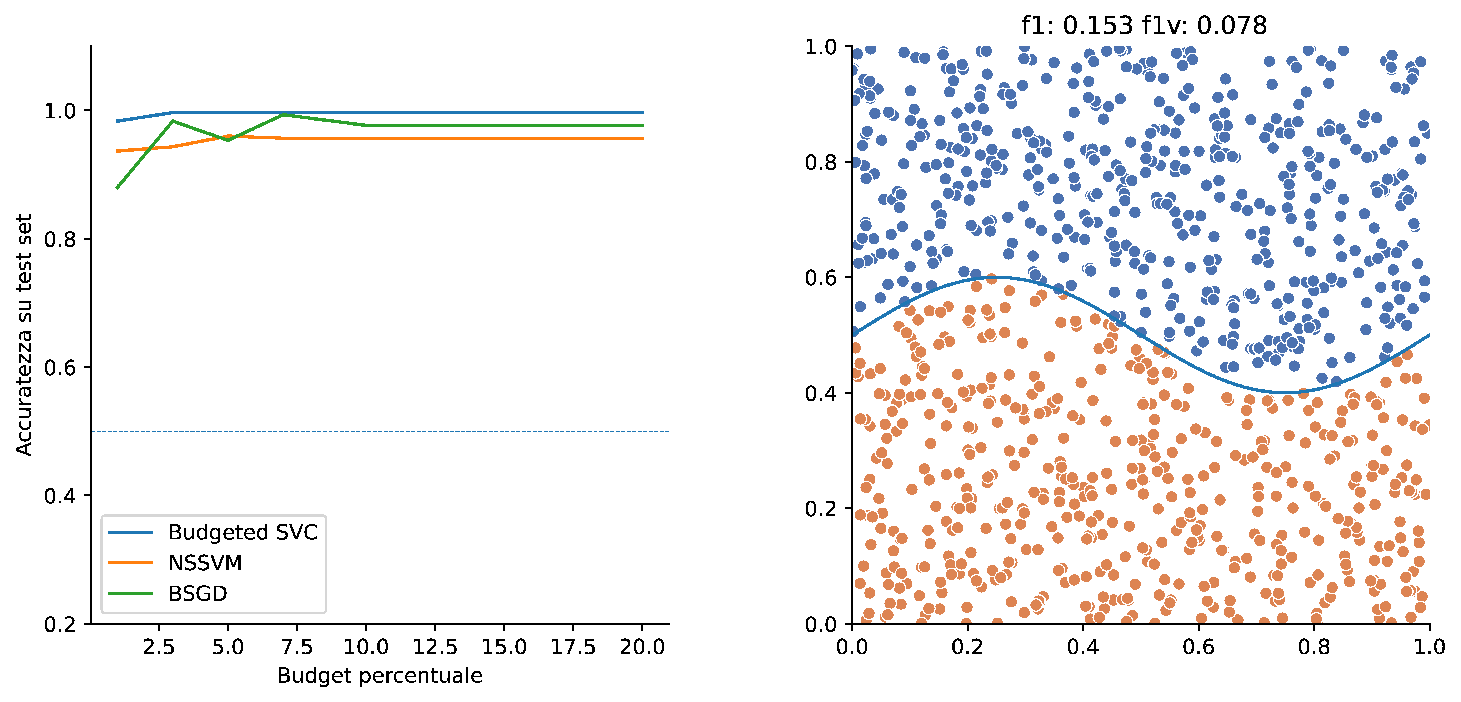
\includegraphics[width=\textwidth]{img/comp_new/10.pdf}
    \end{subfigure}%
    \hfill
    \begin{subfigure}{.8\textwidth}
        \centering
        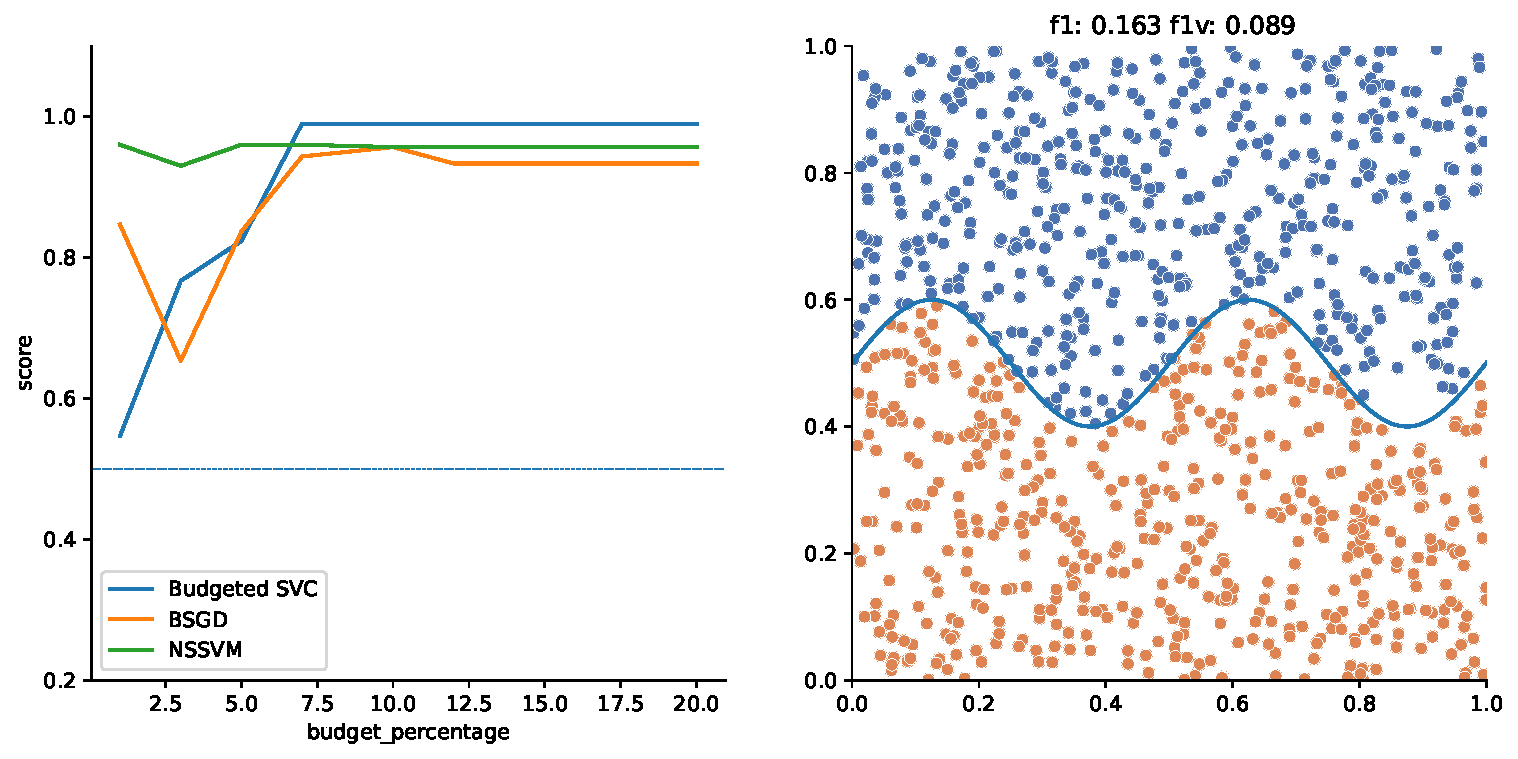
\includegraphics[width=\textwidth]{img/comp_new/11.pdf}
    \end{subfigure}
    \hfill
    \begin{subfigure}{.8\textwidth}
        \centering
        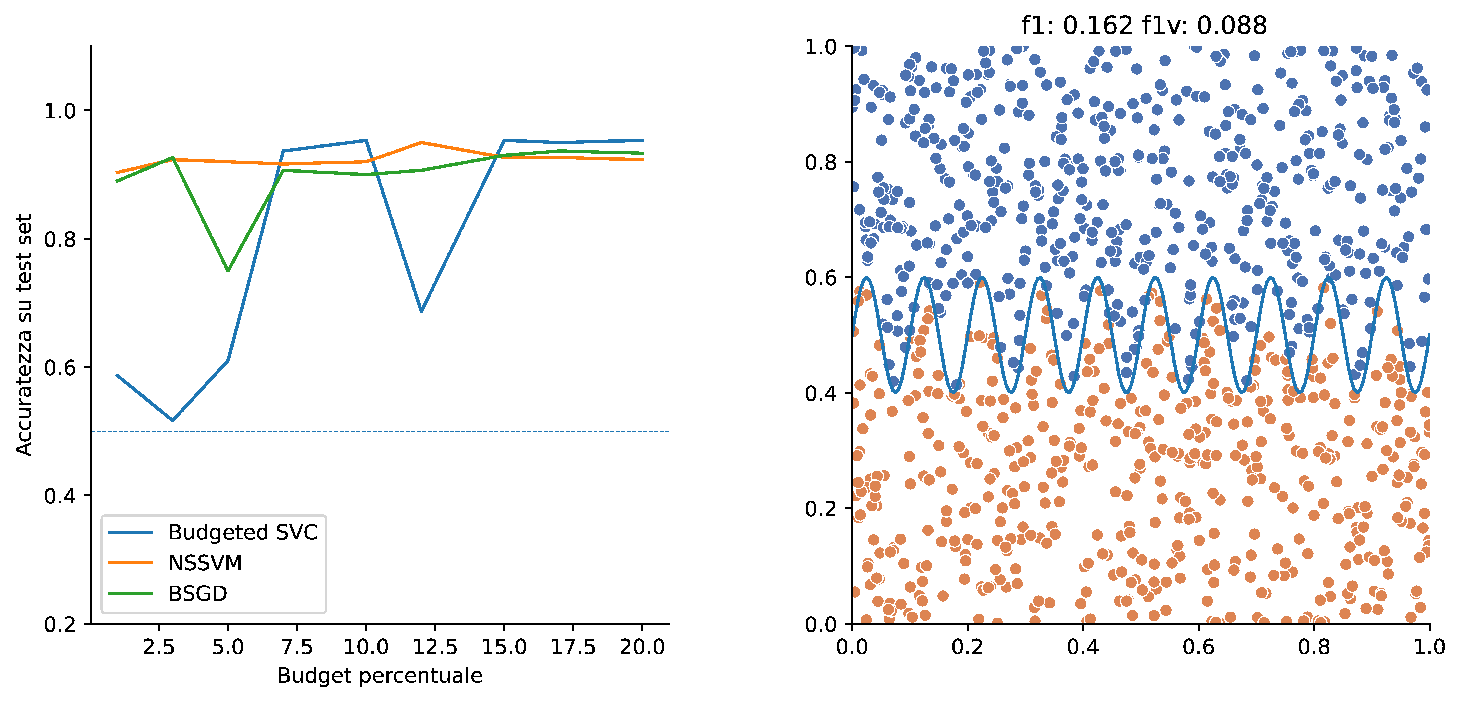
\includegraphics[width=\textwidth]{img/comp_new/13.pdf}
    \end{subfigure}
 \caption[Risultati su \emph{dataset} sintetici utilizzando strategia 2 in confronto ad altri metodi.]{Questi grafici completano la~\Cref{fig:comp_new}. Risultati ottenuti su \emph{dataset} sintetici bidimensionali utilizzando la strategia 2, analogo ai risultati in~\Cref{fig:2d_v2} ma con una curva per ogni metodo utilizzato: la proposta \emph{Budgeted SVC}, i metodi \emph{NSSVM} e \emph{BSGD}.}

\end{figure}


\end{appendices}